% $Id: opus-core.tex,v 1.96 2007/06/01 23:49:22 borning Exp $

% Copyright (c) 2005-2007 Center for Urban Simulation and Policy Analysis,
% University of Washington.  Permission is granted to copy, distribute and/or
% modify this document under the terms of the GNU Free Documentation License,
% Version 1.2 or any later version published by the Free Software Foundation;
% with no Invariant Sections, no Front-Cover Texts, and no Back-Cover Texts.
% A copy of the license is included in the section entitled "GNU Free
% Documentation License".

\chapter{The \package{opus_core} Opus Package}

%\emph{This section should walk through the Opus architecture, how it is
%organized into packages, and where those are located on the file system.
%Discuss where users should put their own scripts and data, and how they get
%access to them.}

%\section{Structure}

Opus is organized as a set of ``Opus packages''.  Each Opus package
encapsulates a set of functionality in a structure defined by a set of
required directories and files.  
%Opus will have simple mechanisms to create a
%new package, bundle a package for distribution, and install or uninstall a
%package. 
This chapter describes main objects provided by the Opus
package called \package{opus_core}. This package is intended to provide 
a fairly general functionality, including data representation and manipulation, 
various models for use in different domains, support for specification of models,
or definition of variables. The package by itself does not provide a self-contained
system of configured models that would run after pressing a button. It is rather a 
collection of tools for building other opus packages.


\section{Datasets}
\label{sec:opus-core-datasets}
%
The basic class for dealing with data is called \class{Dataset}.
\datasetindex 
A dataset \datasetindex is a collection of attributes \attributesindex for a particular type of entity,
such as a set of grid cells, or a set of households.  Each member in this set
has the same set of characteristics, such as income of households.  In Opus,
these characteristics are called attributes. \attributesindex

Conceptually, a dataset \datasetindex is similar to a table.  Each attribute \attributesindex is a column.
Each row describes the attribute values for one member of the dataset. \datasetindex

Some attributes \attributesindex are read from a data store, we call them {\it primary
  attributes}. \primaryattributesindex  Others, {\it computed attributes}, \computedattributesindex are computed by Opus
variable definitions.  Attributes \attributesindex can be also modified or created by models.

In this section, we describe the main functionality of \class{Dataset}. For a list of additional methods, 
see Appendix~\ref{app:selected-methods-dataset}.

%
\subsection{Initialization}
%
The \class{Dataset} \datasetindex class is initialized by the following arguments:
\begin{description}
\item[resources] \index{resources} - on object of class \class{Resources}\index{Resources} (dictionary). It can
  contain any of the remaining arguments, but if an argument of the
  constructor is not None, it has a priority over the entry in
  \verb|resources|.
\item[in_storage] \index{in_storage} - an object of class \class{Storage}\index{Storage} for reading the data
  from (see Section~\ref{sec:data-storage}).
\item[id_name] \index{in_name} - a list of character strings giving the names of the unique
  identifiers of the dataset. \datasetindex If it is an empty list, a ``hidden'' identifier\index{hidden identifier}
  will be created, i.e. an additional attribute of the dataset that enumerates the entries.
\item[dataset_name] \index{database_name} - a character string giving the name of the dataset. \datasetindex
\item[out_storage] \index{out_storage} - an object of class \class{Storage}\index{Storage} for writing the data
  into (see Section~\ref{sec:data-storage}). This argument can be omitted in
  the constructor and instead directly passed to the
  \method{write_dataset()} method, which is the only method of the class that uses this argument.
\item[in_table_name] \index{in_table_name} - name of the table, directory or file that contains the
  data for this dataset \datasetindex (see Section~\ref{sec:data-storage} for the different
  meanings of this argument in the different storage classes).  This name also is the
  name used for this dataset \datasetindex in the cache (see below).
\item[out_table_name] \index{out_table_name} - name of the table, directory or file that the dataset \datasetindex
  should be written into (see Section~\ref{sec:data-storage} for the different
  meanings of this argument in the different storage classes). This argument
  can be omitted in the constructor and instead directly passed to the
  \method{write_dataset()} method.
\end{description}

All arguments are merged with \verb|resources| and kept in the class attribute \attributesindex
\verb|resources|.

The constructor determines all attributes \attributesindex available on the input storage
(primary attributes), \primaryattributesindex without loading them into memory. If \verb|id_name|
is an empty list, it loads at least one attribute \attributesindex from the storage in order to
obtain the dataset \datasetindex size. The constructor also sets up a reference to the
singleton \class{AttributeCache} which is used for caching data (see below).

%
\subsection{Loading Attributes}
\index{Memory!Lazy loading of attributes}
%
Primary attributes \primaryattributesindex are read lazily, i.e.\ they are loaded from the input
storage as they are needed, for example when they are required by a model or
by a variable definition. The loading can be also explicitly invoked by the
method \method{load_dataset()} \datasetindex which by default loads all attributes \attributesindex found on
the data storage. An optional argument \verb|attributes| \attributesindex can be passed which
is a list of attributes \attributesindex to be loaded.

Alternatively, the method \method{get_attribute(name)} \attributesindex invokes the specified
attribute \attributesindex to be loaded into memory if it has not been done before and returns
an array of values for this attribute. \attributesindex Note that when using a slow storage,
such as MySQL, loading several attributes \attributesindex at once using \method{load_dataset()} \datasetindex
(as opposed to one by one using \method{get_attribute()}) \attributesindex might be more
time efficient. \index{Memory management!Using multiple chunks per model}

Loaded or computed dataset \datasetindex attributes \attributesindex can be flushed into a simulation cache to
save memory \index{Memory!Flushing attributes} (using method
\method{flush_attribute(name)} \attributesindex for a specific attribute \attributesindex or
\method{flush_dataset()} for the whole dataset). \datasetindex Opus uses an FLT storage for
the simulation cache (see Section~\ref{sec:flt-storage}) which deals with
reading and writing data in a very efficient way. Thus, when using a slow
storage, it might be of an advantage to load the whole dataset \datasetindex at the beginning
of the dataset \datasetindex usage and flush all attributes. \attributesindex Then any subsequent load will be
performed on the fast cache.

\subsection{Attribute Names}
\label{sec:opus-core-attribute-names}
%
Attributes \attributesindex for a dataset \datasetindex can be specified in following ways:

\begin{description}
\item[Un-qualified name] (e.g.\ \code{population}) It is a character string
  without any dots or parentheses. It may contain numbers. Un-qualified
  names within a dataset \datasetindex must be unique. This way of
  specifying attributes \attributesindex may be used only for accessing
  already existing attributes \attributesindex within a dataset,
  \datasetindex e.g.  in the method
  \verb|get_attribute()|. \attributesindex

\item[Dataset-qualified name] (e.g.\ \code{gridcell.population}) Specifies
  a primary attribute \attributesindex of a specific dataset. \datasetindex
  It consists of a dataset \datasetindex name (e.g.  \verb|gridcell|) and
  an un-qualified attribute \attributesindex name (e.g.
  \verb|population|).  The dataset \datasetindex name allows you to
  disambiguate attributes \attributesindex of the same name in different
  datasets, \datasetindex when using outside of a dataset, \datasetindex
  e.g. in a model specification or in variable \variablesindex
  dependencies.

\item[Fully-qualified name] (e.g.\ \code{urbansim.gridcell.population})
  Specifies an Opus variable. \variablesindex It is the full name of the
  module or class in which the variable \variablesindex is defined. See
  Section~\ref{sec:variable-names} below, for more information.

\item[Expression] (e.g.\ \code{ln(urbansim.gridcell.population+1)})
  \index{expressions}
  Expressions are composed from variable names, constants, functions, and
  operators --- see Sections \ref{sec:urbansim-tutorial-expressions} and
  \ref{sec:opus-core-expressions}.

\end{description}
Expressions and fully-qualified names can be given an alias using the syntax
\verb|alias = expr|.  In that case, the alias name is used as un-qualified
name for this attribute and thus, values of this attribute can be accessed
by \verb|get_attribute(alias)|.

%
\subsection{Computing Variables}
%
A variable (or equivalently, a computed attribute) is specified either by an expression of by a 
fully-qualified name (see Section~\ref{sec:opus-variable}).
Datasets \datasetindex automatically compute each variable \variablesindex when, and only when,
needed. \index{Lazy evaluation}  This mechanism uses the dependency information
from each variable \variablesindex which gives an information about what variables \variablesindex this
variable \variablesindex depends on. Additionally, it is checked if variable's \variablesindex dependent
variables \variablesindex have changed (versioning mechanism).  The computation is invoked by
the dataset \datasetindex method \method{compute_variables()} which computes each of the
given variables \variablesindex if either (a) this variable \variablesindex has not been computed before, or
(b) the inputs to this variable \variablesindex (the values of variables \variablesindex upon which this
variable \variablesindex depends) have changed since the last computation.  Thus, invoking
\method{compute_variables()} \variablesindex on a single variable \variablesindex may either result in no more
computation, or have a ripple effect of computing many variables \variablesindex upon which
this one variable \variablesindex depends.  Lazily computing variables \variablesindex both helps minimize the
computational load as well as eliminating the need to worry about when
variables \variablesindex are computed: it will happen when, and only when, it is needed.

The method \method{compute_variables()} \variablesindex takes as an arguments a list of
variable \variablesindex names to be computed and an object of class \class{DatasetPool} which
maintains a 'pool' of additional datasets that the variables \variablesindex (and their dependent
variables) \variablesindex need for the computation (see Section~\ref{sec:core-dataset-pool}). 
The method returns an array of values that result from computing the last variable in the 
list of variable names.

\subsection{Visualizing Datasets}
%
Opus offers a few methods for plotting values of a dataset. \datasetindex They usually
require specific libraries to be installed, such as matplotlib (see your
Installation directions at your \file{opus_docs/docs/install.html}).

\subsubsection{One-dimensional Plots}
%
Attributes \attributesindex in a dataset \datasetindex are stored as one-dimensional arrays, thus they can be
plotted for example as a histogram \histogramindex or as a scatter plot. \scatterplotindex The \class{Dataset} 
offers the following methods:

\begin{description}
\item[\method{plot_histogram(name, ...)}] \histogramindex creates a histogram \histogramindex of attribute \attributesindex
\verb|name| using matplotlib. \matplotlibindex
\item[\method{r_histogram(name, ...)}] \rindex\histogramindex creates
such histogram \histogramindex including a density line using the rpy \rpyindex library.
\item[\method{plot_scatter(name_x, name_y, ...)}] \rindex\scatterplotindex creates a scatter plot \scatterplotindex for two
attributes \attributesindex using matplotlib. \matplotlibindex
\item[\method{r_scatter(name_x, name_y, ...)}] \rindex\scatterplotindex creates a scatter plot \scatterplotindex 
using the rpy \rpyindex library.
\end{description}

\subsubsection{Two-dimensional Plots}
%
One often is interested in a spatial graphical presentation of a dataset
attribute.  By default, datasets have no spatial coordinate axes.  If you want
a dataset to have a coordinate system, set the dataset's class attribute
\verb|_coordinate_system| to be a tuple of the attribute names for the x and y
coordinates, e.g. to \verb|('relative_x','relative_y')|.  This information then
will be used by routines that need it.

\begin{description}
\item[\method{plot_map(name, ...)}] creates an image using the matplotlib \matplotlibindex
library.
\item[\method{r_image(name, ...)}] \rindex does the same using the rpy \rpyindex
library.
\item[\method{openev_plot(name, ...)}] \openevindex uses OpenEV \openevindex for creating the
  image.
\end{description}

\subsection{Attribute Box}
\label{sec:attribute-box}
%
For each attribute \attributesindex that is loaded into memory or computed, the dataset \datasetindex creates
an instance of \class{AttributeBox}. \attributesindex This object holds all information
about the attribute, \attributesindex such as the data, attribute \attributesindex name, 
version, type, if it is cached or in memory, and a corresponding
instance of class \class{Variable} \variablesindex if this attribute \attributesindex is a variable. \variablesindex This
information can be accessed by the \class{AttributeBox} \attributesindex methods
\method{get_data()}, \method{get_variable_name()}, \variablesindex \method{get_version()},
\method{get_type()}, \method{is_cached()}, \method{is_in_memory()},
\method{get_variable_instance()}. \variablesindex The attribute \attributesindex box for a particular attribute \attributesindex
can be accessed by the dataset \datasetindex method
\method{_get_attribute_box(attribute_name)}, \attributesindex where the \verb|attribute_name| \attributesindex is
given in one of the  forms from Section~\ref{sec:opus-core-attribute-names}.

\subsection{Subsets of Dataset}
\datasetindex\datasetsubsetindex
%
Opus implements a child class of \class{Dataset}, \datasetindex called \class{DatasetSubset}, \datasetsubsetindex
which allows to define a subset of a dataset. \datasetindex\datasetsubsetindex Conceptually, it is a viewing
window for the parent \class{Dataset} \datasetindex object, not a copy. Thus, any change in
the parent object is seen by the child.

It is initialized by passing the parent object and an index to the
constructor.  The index determines indices of elements within the parent
object that should be seen. Any call of \method{get_attribute()} \attributesindex on the subset returns
values corresponding to the index.
A subset can be also created using the \class{Dataset} method {\method{create_subset_window_by_ids(ids)}
called on the parent object. 

Note that only methods for viewing attributes (such as \method{get_attribute()} or \method{summary()}) make sense
for using with a subset. Other
methods that would for example modify attributes (such as \method{compute_variables()}) could destroy the parent dataset.

\subsection{Interaction Sets}
\label{sec:interaction-set}
%
Opus allows the programmer to create a dataset representing
an interaction between two datasets, \datasetindex by using the class
\class{InteractionDataset}, which is a child of \class{Dataset}. \datasetindex It serves mainly
to enable the use of the Opus variable \variablesindex concept for variables \variablesindex
that are defined as an interaction between datasets, \datasetindex and thus are of a 2-d
shape. The class does not support loading from and writing into a storage.

\subsubsection{Initialization}
The class is initialized by the following arguments:
\begin{description}
\item[resources] - this argument has the same meaning as in \class{Dataset}. \datasetindex
\item[dataset1] - an instance of \class{Dataset}. \datasetindex
\item[dataset2] - an instance of \class{Dataset}. \datasetindex
\item[index1] - indices of \verb|dataset1| over which the interaction is
  done. If it is not given, all elements are taken.
\item[index2] - indices of \verb|dataset2| over which the interaction is
  done. If it is not given, all elements are taken.
\item[dataset_name] - a name of the interaction set. Default value is the
  dataset \datasetindex name of  \verb|dataset1| connected by `_x_' to the dataset \datasetindex name of
  \verb|dataset2|.
\end{description}

\subsubsection{Using InteractionDataset}
%
The method \method{get_attribute()} \attributesindex returns a 2-d array, where a value
$x_{ij}$ belongs to interaction of the $i$-th element within elements of
\verb|dataset1| given by \verb|index1| and the $j$-th element within
elements of \verb|dataset2| given by \verb|index2|. Thus, the array size
corresponds to size of \verb|index1| $\times$ size of \verb|index2|.

The two interacting datasets \datasetindex can be accessed by the method
\method{get_dataset()} which takes either 1 or 2 as an argument value for
\verb|dataset1| or \verb|dataset2|.

The method \method{get_attribute_of_dataset(name, dataset_number)} returns values of
the given attribute \attributesindex that belongs to the dataset given by  \verb|dataset_number| where
only values associated to the corresponding index are included. Thus, a
call \verb|self.get_attribute_of_dataset("attr", 1)| \attributesindex gives an array of size
\verb|index1|, whereas a call \verb|self.get_dataset(1).get_attribute("attr")| \attributesindex
gives an array containing values for all elements of \verb|dataset1|.

The method \method{compute_variables()} \variablesindex determines from the fully-qualified
names of variables, \variablesindex to which dataset the variable \variablesindex belongs to. If it belongs to
the \verb|dataset1| or \verb|dataset2|, it calls \method{compute_variables()} \variablesindex on
those datasets (the values are computed for all elements of the datasets,
regardless of the given index). If it is an interaction variable, \variablesindex it is
computed only for elements given by \verb|index1| and \verb|index2|.

The \class{InteractionDataset} class contains several methods that are useful for
variable \variablesindex computation, such as \method{multiply()} and \method{divide()}.

An interaction set is automatically created and used in the
\class{ChoiceModel} class (see Section~\ref{sec:choice-model}).

\section{Data Storage}
\label{sec:data-storage}
%
One of the design elements of Opus is to allow users to choose alternative
data storage methods depending on their needs, while keeping a consistent
internal representation of data used by the system.  Currently Opus classes
exist for reading and writing data in Random Access Memory (RAM), to database
tables, Tab-delimited ASCII files, and binary files.  Other storage methods can
be added as the need arises.

The generic class that supports data storage is called
\class{Storage}. Every class that we describe below derives from this class and
implements the storage interface. All such classes therefore provide the
following methods:

{\bf \method{load_table()}}: Loads the data stored in the data repository and
returns it as a dicionary, where each key represents an attribute (column) of
the table. The only required argument is \verb|table_name|. Optional
arguments include \verb|column_names| (a list of columns that you want loaded;
the default is to load all) and \verb|lowercase| (for forcing all names column
names to lowercase). 

{\bf \method{write_table()}}: Writes data out to the respective storage. The
two non-optional parameters are \verb|table_name| and \verb|table_data|, the
former naming the table and the latter defining the data to be written. More
specifically, the \verb|table_data| argument should be a dictionary, where
the keys represent a column and the values represent the data in those columns. 
This is the same format as that returned by the \method{load_table()} method.
An optional parameter \verb|mode| allows you to determine whether an existing
table of the same name will either be overwritten or appended to with the new
data. By default the table is overwritten. 

{\bf \method{get_storage_location()}}: Returns the location at which data is
being stored for this storage object. In the case of storage locations that
exist on disk, a file path is returned. In the case of a database, an
\class{OpusDatabase} object will be returned. 

{\bf \method{get_column_names()}}: Takes a \verb|table_name| as an
argument and returns a list of attribute names that were found on the storage.

{\bf \method{table_exists()}}: Takes a \verb|table_name| as an
argument and returns whether a table by that name exists at the respective
storage location.

{\bf \method{get_table_names()}}: Returns a list of all the names of tables
that exist at the respective storage location.

{\bf Developer note:} {\textit In order to be able to implement the storage
interface, the new storage subclass must implement methods \method{load_table},
\method{get_storage_location}, \method{write_table},
and \method{get_column_names}.}

The predefined storage classes in \package{opus_core} are \class{dict_storage}, \class{csv_storage},
\class{tab_storage}, \class{sql_storage}, \class{flt_storage}, and \class{dbf_storage} implemented
in modules of the same name in \verb|opus_core.store|. Their instances can be
created using the method \method{get_storage(type, storage_location,...)} of
class \class{StorageFactory}; \verb|type| is the storage type (e.g. ``sql_storage'')
and \verb|storage_location| is either a location on disk or an
\class{OpusDatabase}, depending on the type of storage being created.
Other optional, storage-type specific arguments can also be passed in to the
\method{get_storage} method. We now give a brief description of each available
storage type, and how each may deviate from the above descriptions. 

\subsection{dict_storage}
\label{sec:ram-storage}
%
The simplest storage class. It is an in-memory implementation of the
storage interface. The constructor of this class has no parameters (no \verb|storage_location|
parameter needed).

\subsection{csv_storage and tab_storage}
%
Both \verb|csv_storage| and \verb|tab_storage| provide file-based storage.  
They are based upon Python's csv module, and thus will appropriately
format data as necessary.

The constructor of this class expects an entry \verb|storage_location| in its
arguments. It should be a base directory on a hard drive where
the data will be stored to and loaded from.

For these storage classes, all implemented methods of the storage interface which
accept a \verb|table_name| parameter interpret it as a file name without
extension (relative to the base directory) in which the data is stored (or where
it should be stored). The extension is added automatically. The data is stored
with one attribute per column. The first row contains the attribute names and
optional type information for each column. The type information, if provided, is
appended to the column name and separated by a colon, as in \verb|id:int32| which
specifies to use the numpy \verb|int32| type for storing the \verb|id| values. 
The type may be any of the numpy types in
Table~\ref{storage-numpy-python-mapping}:


\begin{table}
\begin{center}
\begin{tabular}{|l|}\hline
Storage Type \\
\hline
bool8 \\
int8 \\
uint8 \\
int16 \\
uint16 \\
int32 \\
uint32 \\
int64 \\
uint64 \\
float32 \\
float64 \\
complex64 \\
complex128 \\
\hline
\end{tabular}
\end{center}
\caption{\label{storage-numpy-python-mapping}Allowable column types
for csv_storage and tab_storage.}
\end{table}

If type information is not included, Opus will use \verb|float64| for numeric data
and \verb|string| for string data.

For instance, the \verb|csv_storage| for a dataset with three attributes
\verb|a|, \verb|b|, and \verb|c| containing two rows of data could look like:

\begin{verbatim}
a:int8,b:float32,c:string40
1,3.14,hello
2,2.18,there
\end{verbatim}

% The method \method{write_dataset()} writes the data to the file whose name is
% constructed by appending a to the \verb|out_table_name| entry in
% the \verb|write_resources| argument to \method{write_dataset()}.
% \verb|csv_storage| uses the ``csv'' suffix.  \verb|tab_storage| uses the
% ``tab'' suffix.  \method{write_dataset()} always appends type information to
% the column names.


\subsection{sql_storage}
\label{sec:sql-storage}
%
The constructor of this class expects an entry \verb|storage_location| in its
arguments. This parameter should be an \class{OpusDatabase} and it governs a
connection to a database. Here's an example of obtaining an
\class{OpusDatabase} and then creating a storage object that can read and write from that database:

\begin{verbatim}
>>> import os
>>> from opus_core.database_management.database_server_configuration import DatabaseServerConfiguration
>>> from opus_core.database_management.database_server import DatabaseServer
>>> from opus_core.storage_factory import StorageFactory
>>> config = DatabaseServerConfiguration(hostname = os.environ["MYSQLHOSTNAME"],
                                         username = os.environ["MYSQLUSERNAME"],
                                         password = os.environ["MYSQLPASSWORD"],
                                         protocol = "mysql")
>>> db = DatabaseServer(config).get_database(database_name = ``mydatabase'')
>>> storage = StorageFactory().get_storage('sql_storage',
        storage_location = db)
\end{verbatim}

Note that the parameters \verb|hostname|, \verb|username|, and
\verb|password| to \class{DatabaseServerConfiguration} are actually only
necessary if you are trying to connect to a database that cannot be accessed via the server
information that you have specified in your environment variables. Protocol
will default to ``mysql'', unless you have set your DEFAULT_URBANSIM_DB_ENGINE
environment variable to another database engine (e.g. postgres). 

Now you have obtained a \class{sql_storage} object. For this storage class,
all implemented methods of the storage interface which accept a \verb|table_name| parameter interpret it as
name of a table in the database which is to be read from or written to,
depending on the method.

\subsection{flt_storage}
\label{sec:flt-storage}
%
As in the case of tab storage, the constructor expects an entry
\verb|storage_location| in its argument. It is the base
directory where the data are stored to and loaded from.

For this storage class, all implemented methods of the storage interface which
accept a \verb|table_name| parameter interpret it as a subdirectory in the base
directory in which each attribute is stored as a single file in a binary format.
The file names correspond to attribute names with an extension that determines
the type of the stored data. The file extension consists of three parts, one
character for the byte order, one character for the type of the data, and one or
more characters for the size of the column in bytes. The extension is similar to
the dtype for numpy arrays, only the charakter for the byte order is changed from
'<', '>', or '|' (for little endian, big endian, or irrelevant) to 'l', 'b', or
'i'. The method \method{write_table()} stores attribute according to the scheme
above.

\subsection{dbf_storage}
%
The \verb|dbf_storage| provides DBase-formated file-based storage for
datasets.  It uses the dbfpy Python package available at
\url{http://sourceforge.net/projects/dbfpy">http://sourceforge.net/projects/dbfpy}.

The constructor of this class expects an entry \verb|storage_location| in its
arguments. It should be a base directory on a hard drive where
the data will be stored to and loaded from.

For this storage class, all implemented methods of the storage interface which
accept a \verb|table_name| parameter interpret it as a file name (relative to the
base directory) without an extension in which the data are stored in an ``.dbf''
file.  The extension ``.dbf'' is added automatically. Each table is stored in one
file. The format of these files is described at
\url{http://www.clicketyclick.dk/databases/xbase/format/data_types.html\#DATA_TYPES}.


\section{Opus Variables} \indexii{Variables}{Opus}
\label{sec:opus-variable}
\variablesindex

An Opus variable \variablesindex is an algorithm that provides a value for
each element of a dataset. \datasetindex In most cases, the algorithm
transforms or summarizes existing data.

\subsection{Variable Names}
\label{sec:variable-names}
\variablesindex

A user-defined Opus variable \variablesindex is identified by its
fully-qualified name, such as \verb|urbansim.gridcell.population|.  The
fully-qualified variable \variablesindex name encodes three pieces of
information: the package containing it (e.g., \verb|urbansim|), the name of
the dataset \datasetindex to which this attribute \attributesindex belongs
(e.g., \verb|gridcell|), and the un-qualified name of the variable
\variablesindex which is unique within that dataset \datasetindex (e.g.,
\verb|population|).  Using fully-qualified path names explicitly indicates where
each variable's definition comes from.  (In retrospect, this may not be
ideal, and in the future we may no longer require the package name as part
of variable names.)

Opus contains a class \class{VariableName} \variablesindex that is initialized by passing a
name in one of the forms above. Instances of this class can be also used when
accessing attributes \attributesindex or invoking variable \variablesindex computation.

The similarity to a Python \pythonindex \verb|import| statement is not a
coincidence: Opus uses an \verb|import| statement to load the variable's
\variablesindex definition.

The un-qualified part of an Opus variable \variablesindex name may specify
a ``template'' that matches a family of related variables. \variablesindex
The variable \variablesindex
\verb|mypackage.mydataset.number_of_SSS_projects_within_DDD_meters|, for
instance, matches
\verb|mypackage.mydataset.number_of_residential_projects_within_500_meters|
as well as
\verb|mypackage.mydataset.number_of_industrial_projects_within_1000_meters|.
When Opus looks for the definition of this variable, \variablesindex it
matches any \verb|SSS| to strings of alphabetic characters and underscores,
and any \verb|DDD| to integers. These values are then passed to the
variable \variablesindex code, allowing it to modify its behavior according
to the specified values. When there is an ambiguity, Opus will issue a
fatal error.

Opus variable \variablesindex names must be lower-case, except for any
\verb|SSS| and \verb|DDD| pattern makers.  This reduces the change of
problems with incorrect case, or with migrating Opus code between operating
systems that are case-sensitive and those that are not.

\subsection{Implementation}
\label{sec:variable-implementation}
%
The behavior of each Opus variable \variablesindex is defined in a Python \pythonindex class that is a
child of the generic class \verb|Variable|. \variablesindex The name of the Python \pythonindex module and
class containing the variable \variablesindex implementation must be the same as the
un-qualified part of the Opus variable \variablesindex name, e.g. class \verb|population| is
implemented in file \verb|population.py| for variable \variablesindex
\verb|urbansim.gridcell.population|. The module should be stored in a
directory whose name is the dataset \datasetindex name for which the variable \variablesindex is computed,
in the corresponding package. In the above example, \file{population.py} is
stored in the \verb|gridcell| directory in the top level of the
\package{urbansim} package directory.  This scheme allows Opus to find that
variable. \variablesindex  It also means there may be only one Opus variable per Python \pythonindex
variable \variablesindex module.

\subsubsection{Creating a Variable Object}
\variablesindex\index{Variable!creating}
%
An instance of an existing variable class is
created using the method
\method{get_variable()} \variablesindex\index{VariableFactory!get_variable()}of the
class \class{VariableFactory}. \index{VariableFactory} It takes as arguments
the variable \variablesindex name and the dataset \datasetindex which the variable \variablesindex belongs to. It performs
template matching of the name and invokes the constructor of the corresponding
variable. \variablesindex If there were any templates replaced by \verb|SSS| or \verb|DDD|,
they are passed to the constructor in order as they appear in the name. It
then calls the Variable \variablesindex method \method{set_dataset()} \datasetindex which sets the given
dataset \datasetindex as a class attribute \attributesindex \verb|dataset| \datasetindex of the variable. \variablesindex Thus, using the
Variable \variablesindex method \method{get_dataset()} \datasetindex each variable \variablesindex object has an access to
its ``owner'' dataset. \datasetindex

The \class{VariableFactory} method \method{get_variable()} \variablesindex returns an instance
of the created variable \variablesindex class.

Variable \variablesindex objects are created automatically within the dataset \datasetindex method
\method{compute_variables()} \variablesindex and stored in attribute \attributesindex boxes
(Section~\ref{sec:attribute-box}).

\subsubsection{Required Method \method{compute()}}
\variablesindex\index{Variable!compute()}
%
Each variable \variablesindex class has a required method \method{compute()} which defines how
to compute this variable. \variablesindex

It takes as an argument an object of class \class{Resources}, called
\verb|arguments| which is a container for all arguments and datasets \datasetindex that this
variable \variablesindex might need for its computation. Since this method is called from the
dataset \datasetindex method \method{compute_variables()}, \variablesindex it is important to pass all
required objects into the \verb|resources| argument of
\method{compute_variables()}. \variablesindex If the variable \variablesindex needs attributes \variablesindex of another
dataset, \datasetindex this dataset \datasetindex should be stored in \verb|resources| under its dataset \datasetindex
name.

The implementation of the \method{compute()} method can assume that all
required variables \variablesindex are already computed and accessible by the dataset \datasetindex
method \method{get_attribute()}, \attributesindex if they are listed in the
\method{dependencies()} method (see Section~\ref{sec:dependencies}).

The \method{compute()} method returns a numpy array \numpyindex of the size of number
of elements in the ``owner'' dataset. \datasetindex

\subsubsection{Optional Method \method{dependencies()}}
\index{Variable!dependencies()} \index{dependencies}
\label{sec:dependencies}
%
This optional method takes no arguments and returns a list of variable \variablesindex names
that this variable \variablesindex needs in order to compute its values. Each variable \variablesindex name
must be either a fully-qualified Opus variable \variablesindex name, or a dataset-qualified \datasetindex
primary attribute \primaryattributesindex name. It is important to list all dependent variables \variablesindex
here and don't invoke the computation of the dependent variables \variablesindex from the
\method{compute()} method, since the dependencies tree mechanism would not
work correctly (see Section~\ref{sec:dependencies-tree}). If the names of the
dependent variables \variablesindex are not known at the time this method is called, the
dependencies list can be extended from the \method{compute()} method using the
\class{Variable} \variablesindex method \method{add_dependencies()} which takes as an argument
a list of additional dependencies (specified either as character strings or in
form of \class{AttributeBox}). \attributesindex \method{add_dependencies()} extends the
dependencies list only when the \method{compute()} method runs for the first
time.

\subsubsection{Other Methods and Properties}
%
If the variable \variablesindex defines the property \verb|_return_type| to be one of the
following numpy types, Opus will automatically cast the results into that
type.  If the \verb|arguments| passed into the \method{compute()} method
contains an entry \verb|check_variables|, \variablesindex then it will also issue a warning if
the values being cast are too large to fit into the destination type.  The
allowable values for \verb|_return_type| are:
\begin{itemize}
\tight
\item bool8
\item int8
\item uint8
\item int16
\item uint16
\item int32
\item uint32
\item int64
\item uint64
\item float32
\item float64
\item complex64
\item complex128
\item longlong
\end{itemize}

In addition, each Opus variable \variablesindex may have the optional \method{pre_check()} and
\method{post_check()} methods to implement the ``programming by contract''
\index{Programming by contract} model of software development (see
Section~\ref{sec:programming-by-contract}).

\subsection{Variable Dependencies Tree}
\label{sec:dependencies-tree}
\variablesindex
%
Opus implements a mechanism of computing variables \variablesindex structured in a
dependencies tree. A variable \variablesindex is only computed if its children have changed
since the last computation. Thus, a dataset \datasetindex object keeps a version information
about each attribute \attributesindex or variable \variablesindex and each variable \variablesindex class keeps information
about with which versions of the dependent variables \variablesindex this variable \variablesindex was
computed. This mechanism is automatically invoked by calling the method
\method{compute_variables()} \variablesindex of the class \class{Dataset}. \datasetindex

As an example, consider Figure~\ref{fig:opus-core-variable-tree}. There are 8
variables/attributes, \variablesindex\attributesindex belonging to 3 datasets, \datasetindex \verb|ds1|, \verb|ds2|, and
\verb|ds3|.  The arrows show the dependency hierarchy between variables. \variablesindex The
hierarchy is defined in the method \method{dependencies()} of each variable \variablesindex
where children are listed in their fully-qualified names (in
this example the names in the parentheses in the figure). Note that two
attributes \attributesindex here are primary, namely ``ds3.var_d'' and ``ds2.var_e'', and
thus are defined in their dataset-qualified \datasetindex name (there is no variable \variablesindex
implementation for those attributes). \attributesindex

\begin{figure}
\begin{center}
%begin{latexonly}
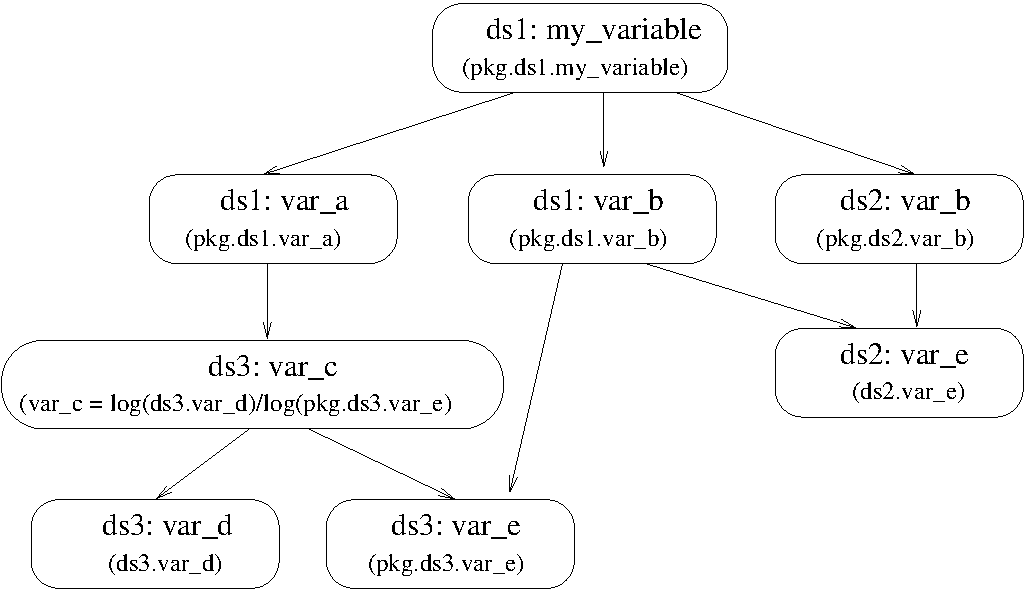
\includegraphics[scale=0.6, angle=-90]{images/variabletreeinitial.pdf}
%end{latexonly}
\caption{\label{fig:opus-core-variable-tree}\small Example of a variable
  dependencies tree.}
\htmlonly{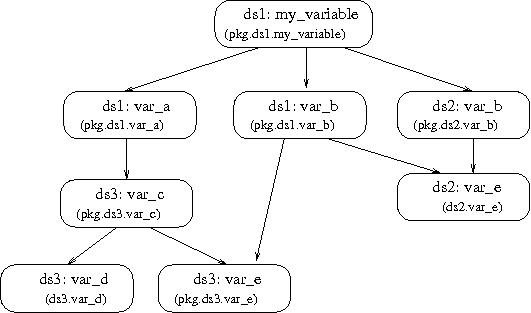
\includegraphics[scale=0.6, angle=-90]{images/variabletreeinitial.jpg}}
\end{center}
\end{figure}

Now suppose we have a system of several models, three of which are invoking
the computation of ``my_variable'' \variablesindex of dataset \datasetindex \verb|ds1|. Suppose also that
initially we have created the three datasets \datasetindex and loaded the two primary
attributes. \primaryattributesindex Opus assigns to each newly created attribute \attributesindex a version number 0 in
its attribute \attributesindex box.  This situation is shown in the left upper corner of
Figure~\ref{fig:opus-core-variable-tree-1}. Box number 1. shows that there are only
two attributes \attributesindex in the system, both with version number 0.

\begin{figure}
\begin{center}
%begin{latexonly}
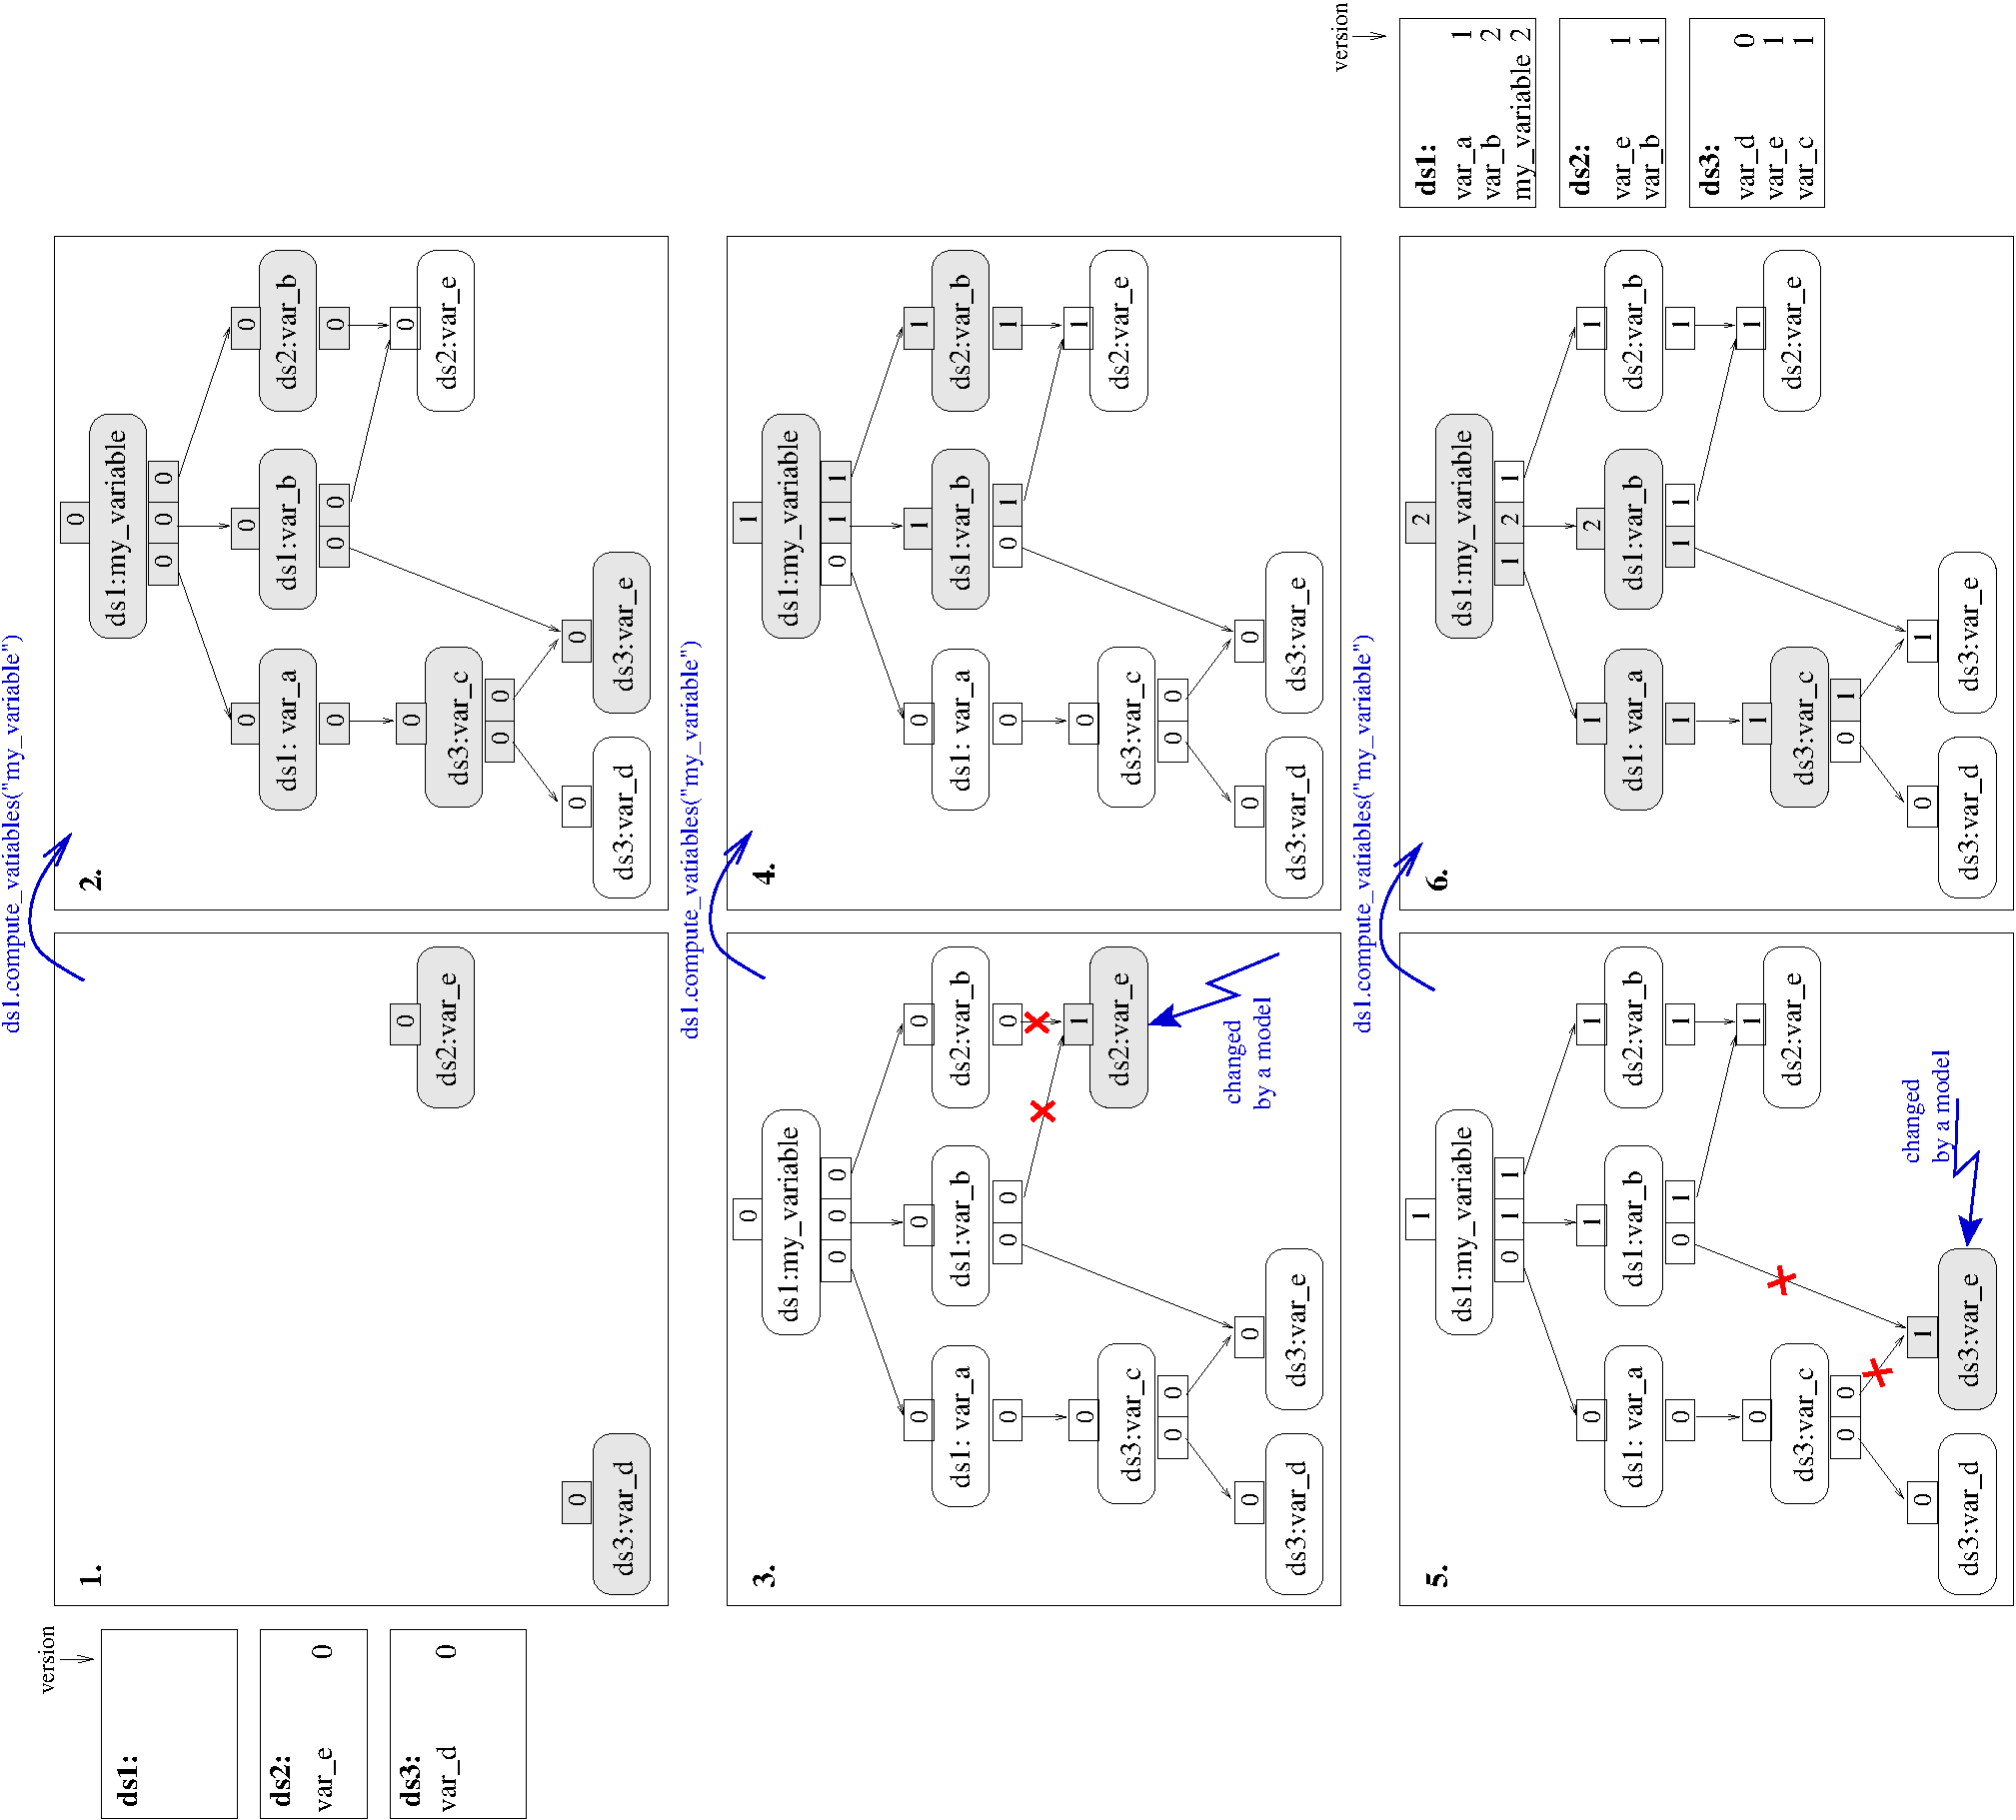
\includegraphics[scale=0.55, angle=-90]{images/variabletree1.pdf}
%end{latexonly}
\caption{\label{fig:opus-core-variable-tree-1}\small Scenario of computing and
  recomputing variables.}
\htmlonly{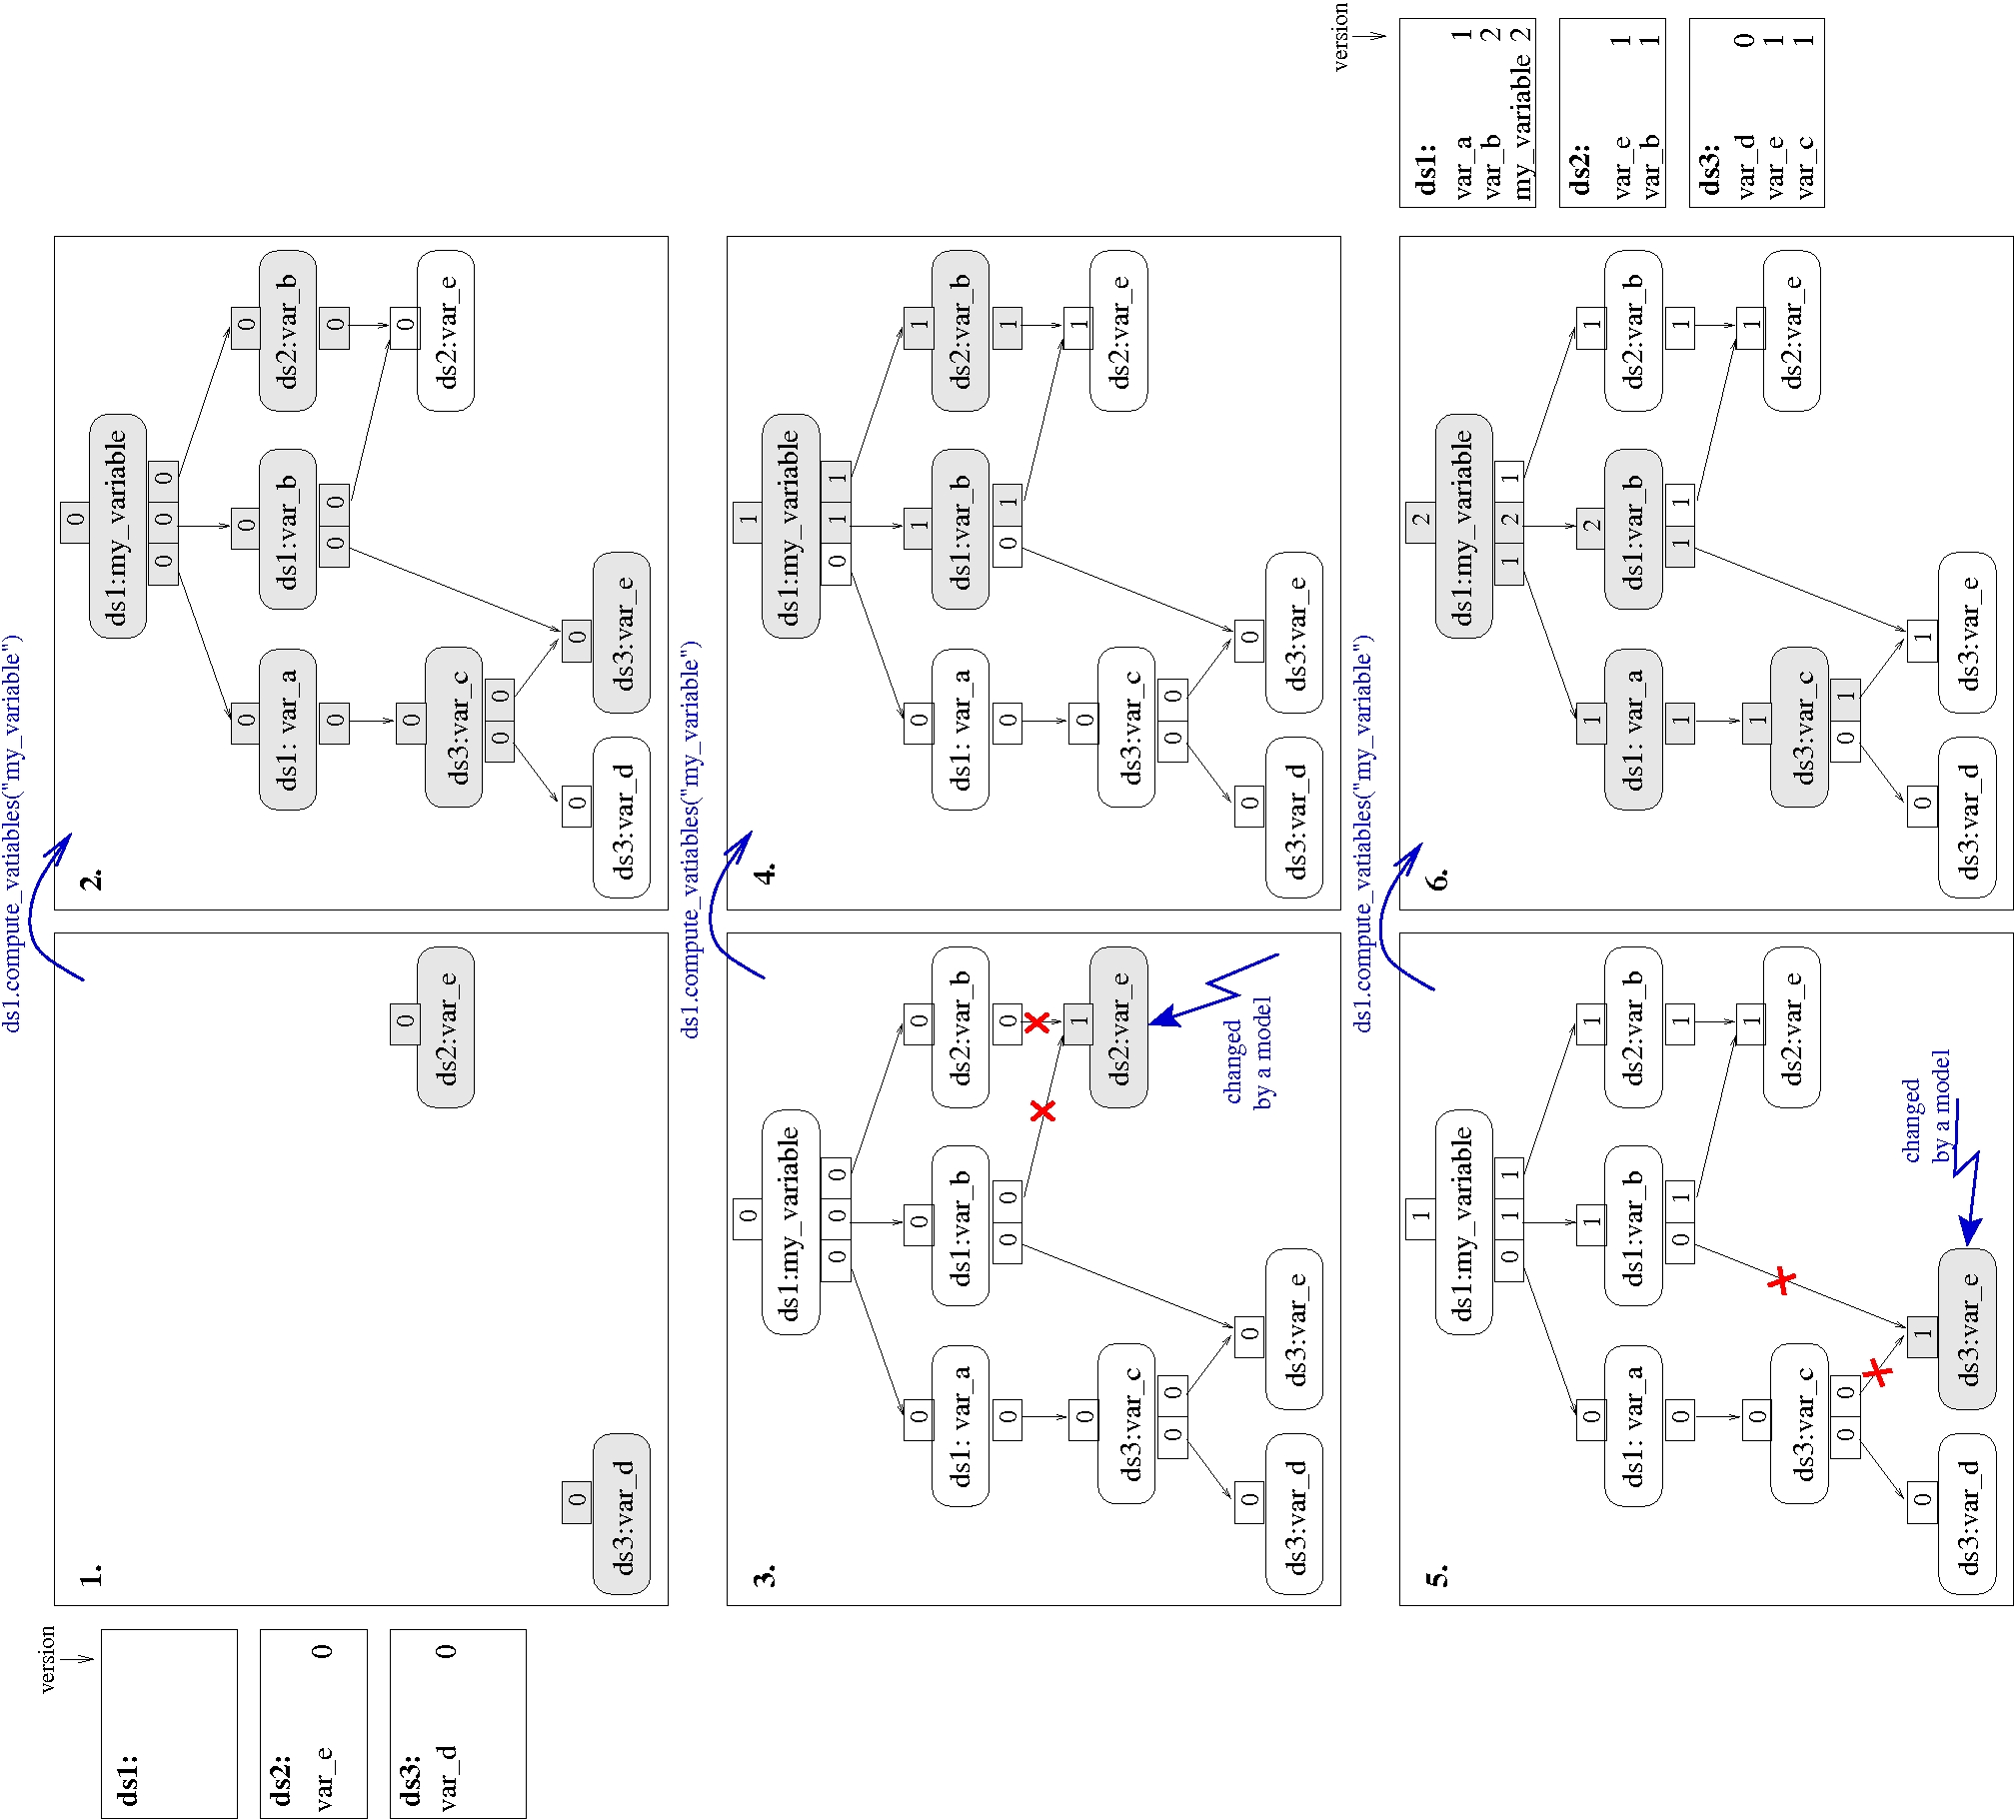
\includegraphics[scale=0.55, angle=-90]{images/variabletree1.jpg}}
\end{center}
\end{figure}

Box 2. shows a situation when the first model invokes the computation of
``my_variable'' \variablesindex \footnote{Because of the dependencies on variables of other
  datasets, the correct call is\\
  \code{ds1.compute_variables("my_variable", resources=Resources({"ds2":ds2, "ds3":ds3}))}.\\
  We simplify it for
  a better readability.}. The system works through the defined dependencies and
computes all variables \variablesindex needed to compute ``my_variable''. \variablesindex In this process,
again, each newly computed variable \variablesindex gets the version number 0 (illustrated by
the small boxes above each variable), \variablesindex stored in the attribute \attributesindex box of each
variable. \variablesindex Additionally, each \class{Variable} \variablesindex instance keeps the version
number for each dependent variable, \variablesindex on which this variable \variablesindex was computed. In
the figure, this is illustrated by the small boxes bellow each variable. \variablesindex
Note that all elements in Figure~\ref{fig:opus-core-variable-tree-1} that are
created or change their values are shaded.

The box number 3. shows a situation in which another model changes values of
variable ``var_e'' of the dataset \datasetindex \verb|ds2| which causes an increment of the
version number. Therefore, when the next model invokes
\method{compute_variables("my_variable")}, \variablesindex Opus determines that there is a
mismatch between versions of ``ds.var_e'' on which variables \variablesindex ``ds1.var_b'' and
``ds2.var_b'' were computed and its current version. Then all
variables \variablesindex above ``ds.var_e'' are recomputed, their version numbers
incremented, and the version numbers in the dependencies lists are updated
(box 4.).

A similar situation arises when another model changes the variable \variablesindex
``ds3.var_e'' (box 5.). The next call of
\method{compute_variables("my_variable")} \variablesindex causes a recomputing of 4
variables \variablesindex (box 6.) In the right lower corner of
Figure~\ref{fig:opus-core-variable-tree-1}, the state of the three datasets \datasetindex is
shown at the end of the run of our example models.

Note that the dependencies tree is constructed using the
\method{dependencies()} method of \class{Variable}. \variablesindex Therefore a missing item
in this method translates to a missing branch of the tree and thus failing to
determine a need for recomputing.

\subsection{Expressions}
\label{sec:opus-core-expressions}
\index{expressions}

In many cases variable definitions are simple expressions involving other
variables.  For these cases, Opus provides an \emph{expression language}
that allows them to be defined succinctly, rather than requiring the Opus
user to write new variable definitions in Python.  The material in this
section is intended to complement that in Section
\ref{sec:urbansim-tutorial-expressions} in Chapter \ref{urbansim-tutorial},
with the Chapter \ref{urbansim-tutorial} material being more tutorial in
nature.

The syntax of the expression language is that of Python, but the semantics
are somewhat different --- for example, a name like
\code{gridcell.distance_to_cbd} is a reference to the value of that
variable; further, expressions are evaluated lazily.

An expression consists of an attribute name, or a function or operation
applied to other expressions.  This definition is recursive, so that a
unary function or binary operator can be applied to expressions composed
from other expressions.

The attribute name used in an expression can be:

\begin{itemize}
\item a fully-qualified variable name (for an existing variable).  Example:
\code{urbansim.gridcell.population}.

\item a dataset-qualified variable name or primary attribute.
Example: \code{household.income}.
\end{itemize}

(Currently the attribute name can also be an un-qualified attribute for an
existing attribute of the dataset, but support for this may be dropped in
future versions of Opus.  So we recommend always qualifying the attribute
name with the name of the dataset in an expression.)

The variable names can include arguments (Section
\ref{sec:tutorial-numbersinvariables}).  For example,
\class{is_near_highway_if_threshold_is_2} matches the variable definition
for \class{is_near_SSS_if_threshold_is_DDD}.

\subsubsection{Unary Functions for Opus Expressions}

The currently available unary functions are listed in Section
\ref{sec:functions-for-opus-expressions}.  These all operate 
on numpy arrays.  The set of available functions can be easily 
extended by adding additional definitions to 
\package{opus_core.variables.functions}.

\subsubsection{Operators for Opus Expressions}
\index{numpy!operators}

All of the numpy operators can be used in Opus expressions, including
\verb|+ - * / ** |.  Note the numpy semantics for these --- for example,
\verb|*| does elementwise multiplication of two numpy arrays, or with a
scalar argument, scales all the elements in an array,
e.g.\ \code{1.2*household.income}.

\subsubsection{Equivalence of Variable Names and Expressions}
\index{expression equivalence}

Two variable names consisting of an attribute, a dataset-qualified
attribute, or a fully-qualified attribute are of course equal if the
component strings are equal.

Two expressions are equal if their defining strings are identical, ignoring
spaces.  Thus these two expressions are equivalent:

\begin{verbatim}
urbansim.gridcell.population+1
urbansim.gridcell.population + 1
\end{verbatim}

However, two textually different expressions are \emph{not} equivalent,
even if they are algebraically equal.  For example,
\verb|1 + urbansim.gridcell.population| is different from the previous
expressions.  In many cases this doesn't matter.  Reasons it may matter
are: (1) if the resulting value uses a lot of memory or takes a long time
to compute, having a second copy of the value will waste memory or
computation time; and (2) if the variable defined by the expression is used
in a specification, you could inadvertently end up with two variables.  For
this reason, good practice is to put each expression that you'll need for a
given package and dataset, along with an alias for that expression, in an
\file{aliases.py} file.  (See Section \ref{sec:aliasing}.)  Elsewhere use
the alias.

\subsubsection{Implementation of Expressions}
\index{expression implementation}

For the most part, the implementation of expressions shouldn't be relevant
to the Opus user.  But for the curious, for programmers who want to extend
the system, or (heaven forfend) in case something goes wrong, here is a
description of the implementation.  The code is in
\package{opus_core.variables}.  

When a new expression is encountered, the system automatically compiles a
new subclass of \class{Variable} that implements the computation defined by
that expression.  If the expression is a simple attribute or
fully-qualified variable, evaluating the expression reduces to getting the
value of the attribute or computing the value of the existing
variable. Otherwise, the expression system generates and compiles a new
variable to implement an expression. It keeps a cache of expressions that
have already been processed, so that autogenerated variables can be reused
when possible. These autogenerated variables have names like
\class{autogenvar034}. They are compiled and live just in the current
process --- they aren't stored on disk, so that the user never needs to see
them, and so that different processes running on the same machine don't
interfere with each other.

Since expressions use standard Python syntax, they can be parsed using the
standard Python parser module, rather than needing to write one. The parse
tree for the expression is analyzed and the dependencies extracted to
generate the dependencies method --- the user doesn't need to declare the
dependencies for an expression. The \method{compute()} method for the
autogenerated variable includes the user's expression directly as part of
the method.  To enable this to work correctly, the method includes
statements to set up the local environment in the method so that all of the
names are properly bound.  Here is an example.  Suppose the input
expression is \verb|ln_bounded(urbansim.gridcell.population)|.  Then the
automatically generated class will be:
\begin{verbatim}
class autogenvar034(Variable):
    def dependencies(self):
        return ['urbansim.gridcell.population']
    def name(self):
        return 'ln_bounded(urbansim.gridcell.population)'
    def compute(self, dataset_pool):
        urbansim = DummyName()
        urbansim.gridcell = DummyDataset(self, 'gridcell', dataset_pool)
        urbansim.gridcell.population = \
            self.get_dataset().get_attribute('population')
        return ln_bounded(urbansim.gridcell.population)
\end{verbatim}

The name of the class is generated (there is a class variable
autogen_number in the class \class{AutogenVariableFactory} that starts at 0
and gets incremented each time it's used in a new name).

The dependencies method is constructed by parsing the expression and
finding all of the other variables that it references, and putting those
into the returned list.

The compute method ends with a return statement that just returns
\code{expr}.  To make this work, we need to provide local bindings for
e.g. \code{urbansim.gridcell.population}.  We bind a local variable (named
\code{urbansim} in the example) to an instance of \class{DummyName}, whose
sole purpose in life is to have an attribute gridcell (and maybe other
attributes if there are multiple dependencies).  Then
\code{urbansim.gridcell} is bound to an instance of \class{DummyDataset},
which is used in place of a real dataset in the autogenerated code.  We
then add a population attribute to \code{urbansim.gridcell}, bound to the
value of the appropriate dataset attribute.  (We use the dummy dataset
rather than adding attributes to the real dataset, which might interfere
with other attributes or not be garbage-collected as soon as they might
otherwise be.)  For the get_attribute call to get the value of the
population attribute, we use the short version of the name -- its value
should already have been computed by virtue of being listed in the
\method{dependencies()} method.

If the expression includes an alias, for example
\verb|pop = ln_bounded(urbansim.gridcell.population)|, then the code is all
the same as above, except that the final return statement is replaced with
\begin{verbatim}
            pop = ln_bounded(urbansim.gridcell.population)
            return pop
\end{verbatim}

The \method{aggregate}, \method{disaggregate}, and \method{number_of_agents}
methods are defined on \class{DummyDataset}, so that they can be used in
expressions.

\section{Models} \index{Models}
\label{sec:opus-core-models}

The \package{opus_core} package offers a few simple models that can serve as parent classes
for user specific models or can be used directly. Their hierarchy is shown in
Figure~\ref{fig:opus-core-model}. \class{Model} and \class{ChunkModel} are abstract
classes, \class{ChoiceModel} and \class{RegressionModel} implement different
model functionality. The classes are described in detail in the next sections.

\begin{figure}
\begin{center}
%begin{latexonly}
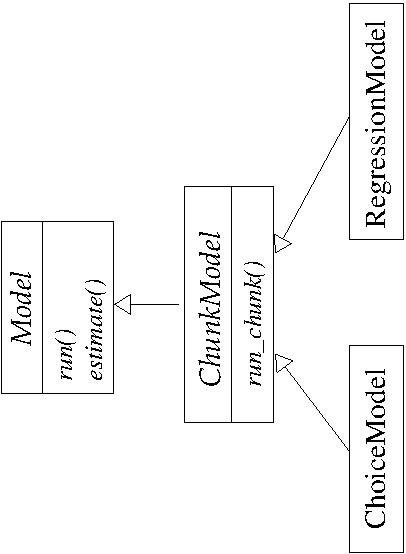
\includegraphics[scale=0.8, angle=-90]{images/coremodelswithmethods.pdf}
%end{latexonly}
\caption{\label{fig:opus-core-model}\small Models in Opus \package{opus_core}.}
\htmlonly{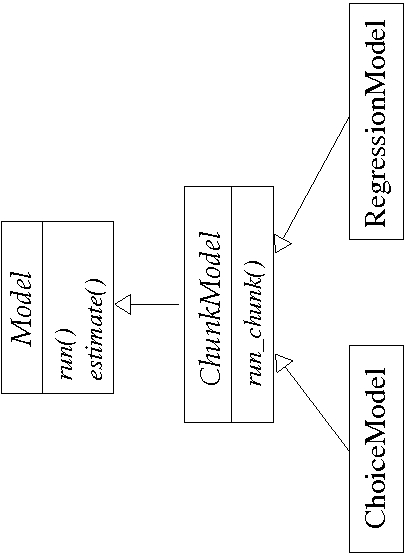
\includegraphics[scale=0.8, angle=-90]{images/coremodelswithmethods.jpg}}
\end{center}
\end{figure}

\subsection{Model Class}
\class{Model} is the base class for implementing Opus models. It provides an
automatic logger which prints out information about the model start, end and
processing time.  Model supports two methods: an obligatory method
\method{run()} and an optional method \method{estimate()}. Each child of
\class{Model} can define a class attribute \attributesindex \verb|models_name| that is used as
an identification of the specific model in the logger output. Any arguments
can be passed into the \method{run()} and \method{estimate()} methods and
those can return any values.

\subsection{ChunkModel Class}
\label{sec:chunk-model} \index{ChunkModel}
\index{Memory management!Using multiple chunks per model}

This class enables running models (i.e. processing the \method{run()} method) in
several chunks, for example if a run of the whole model would require too much
memory. The class does not have any effect on an \method{estimate()} method.

\subsubsection{The Run Method}
{\it Input}:
\begin{description}
\item[chunk_specification] - a dictionary specifying how to determine the number
  of chunks to run the model in (see Section~\ref{sec:models-configuration}).
\item[dataset] - an object of class \class{Dataset} along whose elements the
  model will be chunked.
\item[dataset_index] - an index of elements within \verb|dataset| that are to
  be chunked.
\item[result_array_type] - a type of the resulting array. It can be any numerical type of numpy array. \numpyindex
        The default value is \verb|float32|.
\item[...] - optional additional arguments that are passed to the method
  \method{run_chunk()}. They are expected to be keyword arguments.
\end{description}


{\it Algorithm}:~\\[1mm]
%
For each chunk (determined by the \verb|chunk_specification|) the model calls
the method \method{run_chunk()} and passes as arguments the corresponding portion
of \verb|dataset_index|, \datasetindex the whole \verb|dataset| \datasetindex and all additional
arguments. By default the order of elements in \verb|dataset_index| is
preserved. This can be changed by redefining the method
\method{get_agents_order()}. This method takes a dataset \datasetindex as argument which is an
object of class \class{DatasetSubset} \datasetsubsetindex containing only those elements of the
original \verb|dataset| \datasetindex that are defined by \verb|dataset_index|. \datasetindex It returns
an index of elements in the given dataset \datasetindex determining the order in which the
elements should be processed. For example, if this method returns a randomized
index, the elements passed into \method{run_chunk()} will be processed in
randomized order.


{\it Output}:~\\[1mm]
%
The class returns \verb|result_array| (passed to the method as input) filled
by values returned by \verb|run_chunk()| are filled into. This requires that
the method \verb|run_chunk()| returns an array of the same type as
\verb|result_array| and its size corresponds to the number of elements in one
chunk.

\subsection{ChoiceModel Class}
\label{sec:choice-model}
\index{class!ChoiceModel}
\index{models!choice model}
%
This class implements a functionality of a discrete choice model, an approach
widely used in land use and transportation modeling. In principal, a set of
agents make choices from a finite set of possibilities (alternatives). The
choice selection is based on probabilities derived from utilities. These are
computed on the basis of given variables \variablesindex and coefficients. \coefficientsindex The model allows
the coefficients \coefficientsindex to be also estimated within this framework.

As there are many different aspects to consider in specifying a discrete
choice model, the software has been designed in a modular way to accommodate
substantial flexibility in configuring these models. Each component included
in the model is passed as character string that determines the module$=$class
name (as a fully qualified name) in which the component is implemented.

\subsubsection{Initialization}
%
The class is initialized by passing the following arguments:
\begin{description}
\item[choice_set] - A list, array or dataset \datasetindex that represents the finite set of
  possible choices. It should have numeric values larger than zero.
\item[utilities] - A fully qualified name of the module for computing utilities
  (see Section~\ref{sec:utilities}). Default value is
  \verb|'opus_core.linear_utilities'|.
\item[probabilities] - A fully qualified name of the module for computing
  probabilities (see Section~\ref{sec:probabilities}). Default value is
  \verb|'opus_core.mnl_probabilities'|.
\item[choices] - A fully qualified name of the module for determining
  final choices (see Section~\ref{sec:choices}). Default value is
  \verb|'opus_core.random_choices'|.
\item[submodel_string] - If model contains submodels, this character string
  specifies what agent's attribute \attributesindex determines those submodels.
\item[choice_attribute_name] - Name of the attribute \attributesindex that identifies the
  choices. This argument is only relevant if \verb|choice_set| is not an
  instance of \class{Dataset}. \datasetindex Otherwise the choices are identified by the
  unique identifier of the \verb|choice_set|. Default value is
  \verb|'choice_id'|
\item[interaction_pkg] - This argument is only relevant if there is an
  implementation of an interaction dataset that corresponds to interaction
  between agents and choices. Default value is \verb|'opus_core'|.
\item[run_config] - A collection of additional arguments that control a
  simulation run. It should be of class \class{Resources}.
\item[estimate_config] - A collection of additional arguments that control an
  estimation run. It should be of class \class{Resources}.
\end{description}
The initialization method creates a class attribute \attributesindex \verb|upc_sequence|, using
the passed arguments \verb|utilities|, \verb|probabilities| and
\verb|choices|. It is an object of class \class{upc_sequence} (see
Section~\ref{sec:upc-sequence}). A class attribute \attributesindex \verb|choice_set| is an
object of \class{Dataset}. \datasetindex If the argument \verb|choice_set| is a list or
array, a \class{Dataset} \datasetindex is created using the values of the argument as the
unique identifier called \verb|choice_attribute_name|. \attributesindex

\subsubsection{The Run Method}
%
The \method{run()} method runs the simulation on basis of a given specification
and coefficients. \coefficientsindex

{\it Input}:
\begin{description}
\item[specification] - an instance of class \class{EquationSpecification}
  specifying variables \variablesindex to be used in the simulation.
\item[coefficients] - an instance of class \class{Coefficients} \coefficientsindex that contains
  values of coefficients \coefficientsindex to be used in the simulation.
\item[agent_set] - an instance of class \class{Dataset} \datasetindex representing the whole
  set of agents to be used for the variable \variablesindex computation.
\item[agents_index] - an index within the \verb|agent_set| determining which
  agents enter the choice process. If it is not given, all agents are
  considered.
\item[chunk_specification] - a dictionary specifying how to determine the number
  of chunks to run the model in (see Section~\ref{sec:models-configuration}).
\item[data_objects] - a dictionary containing other datasets \datasetindex and arguments
  needed for computing variables. \variablesindex
\item[run_config] - additional \class{Resources} for controlling the
  simulation run.
\end{description}


{\it Algorithm}:~\\[1mm]
The algorithm is implemented in the method \verb|run_chunk()| called from the
parent class \verb|ChunkModel| for each chunk. It overwrites the
\class{ChunkModel} method \verb|get_agents_order()| in a way that it returns a
permutation of the agents indices. Thus, the agents make their choices in a
random order.

The method creates an interaction set between the agent set and the choice
set. It computes all variables \variablesindex given in the specification. Variables \variablesindex that are
specific to one of the datasets \datasetindex are computed on all elements of that dataset, \datasetindex
interaction variables \variablesindex are computed only on elements entering the choice
process. The method then creates the corresponding data matrix using
\verb|agents_index| for selecting the appropriate data values. It runs one
simulation per submodel (for submodels specified in the specification) by
calling the \verb|run()| method of the \verb|upc_sequence| attribute \attributesindex
(see~\ref{sec:upc-sequence}) and passing the data matrix and the coefficients \coefficientsindex
for the corresponding submodel.

{\it Output}:~\\[1mm]
The method returns an array of size \verb|agents_index|, representing the
choices that agents (elements of \verb|agent_set| determined by
\verb|agents_index|) made. Agents whose choice is less equal zero  were
not included in the choice process, for example because they do not belong to
any submodels given in the specification.

\subsubsection{The Estimate Method}
%
The \method{estimate()} method runs an estimation of coefficients \coefficientsindex on basis of
a given specification.

{\it Input}:
\begin{description}
\item[specification] - an instance of class \class{EquationSpecification}
  specifying variables \variablesindex to be used in the estimation.
\item[agent_set] - a \class{Dataset} \datasetindex representing the whole set of agents
  to be used for the variable \variablesindex computation.
\item[agents_index] - an index within the \verb|agent_set| determining which
  agents will be used for the estimation. If it is not given, all agents are
  considered.
\item[procedure] - a character string giving the fully qualified name of the
  estimation procedure. This argument can be also passed via
  \verb|estimate_config| as an entry \verb|'estimation'|.
\item[data_objects] - a dictionary containing other datasets \datasetindex and arguments
  needed for computing variables. \variablesindex
\item[estimate_config] - additional \class{Resources} for controlling the
  estimation run.
\end{description}

{\it Algorithm}:~\\[1mm]
In addition to \verb|agents_index|, the number of agents entering the
estimation can be controlled by an entry \verb|'estimation_size_agents'| in
\verb|estimate_config| which should have a value between $0$ and $1$. It gives
the portion of \verb|agents_index| (or \verb|agent_set| if \verb|agents_index|
is not given) that will be used in the estimation. The indices are then
randomly sampled. The \verb|agent_set| should contain an attribute \attributesindex of the same
name as the unique identifier of the class attribute \attributesindex \verb|choice_set|. Its
values determine the current choices of the agents.

As in the \method{run()} method, an interaction set is created and the
variables \variablesindex given in the specification are computed. Then for each submodel the
corresponding data matrix is built and the \verb|run()| method of the class
given by the argument \verb|procedure| (or alternatively by an entry
``estimation'' in \verb|estimate_config|) is called, passing the data array,
the class attribute \attributesindex \verb|upc_sequence| and \verb|estimate_config| (after
adding entries needed for the estimation) as arguments (see
Section~\ref{sec:estimation-procedure} for more details).  From the returned
dictionary, items ``estimators'', ``standard_errors'', ``other_measures'' and
``other_info'' are extracted. After results from all submodels are collected,
a \class{Coefficient} \coefficientsindex object is created using those extracted values.

{\it Output}:~\\[1mm]
The method returns a tuple of the created \class{Coefficient} \coefficientsindex object and a
dictionary with entries for each submodel equals a dictionary returned by the
\verb|run()| method of \verb|procedure| for that submodel.


\subsection{RegressionModel Class}
\index{class!RegressionModel}
\index{models!regression model}
%
\label{sec:regression-model}
The \class{RegressionModel} class implements a model based on a regression
procedure. In summary, there is a set of observations, whose attributes \attributesindex or/and
variables \variablesindex are used to predict a certain outcome, using some coefficients. \coefficientsindex
Those can be also estimated within this framework.

As in the case of \class{ChoiceModel}, the regression model can be composed by
plug-in modules.

\subsubsection{Initialization}
The class is initialized by passing the following arguments:
\begin{description}
\item[regression_procedure] - a fully qualified name of the module/class in
  which the regression is implemented (see Section~\ref{sec:regression}).
\item[submodel_string] - If model contains submodels, this character string
  specifies what attribute of the observation set determines those submodels.
\item[run_config] - A collection of additional arguments that control a
  simulation run. It should be of class \class{Resources}.
\item[estimate_config] - A collection of additional arguments that control an
  estimation run. It should be of class \class{Resources}.
\end{description}
From the argument \verb|regression_procedure| the initialization method
creates a class attribute \attributesindex \verb|regression|, using
\class{RegressionModelFactory} (see Section~\ref{sec:model-components}).
The remaining arguments are set as class properties.

\subsubsection{The Run Method}
%
The \method{run()} method runs the simulation on basis of a given
specification and coefficients. \coefficientsindex

{\it Input}:
\begin{description}
\item[specification] - an instance of class \class{EquationSpecification}
  specifying variables \variablesindex to be used in the simulation.
\item[coefficients] \coefficientsindex - an instance of class \class{Coefficients} \coefficientsindex that contains
  values of coefficients \coefficientsindex to be used in the simulation.
\item[dataset] \datasetindex - a \class{Dataset} \datasetindex representing the whole set of observations.
\item[index] - an index within \verb|dataset| determining for which
  observations the prediction is to be made. If it is not given, the whole
  \verb|dataset| \datasetindex is considered.
\item[chunk_specification] - a dictionary specifying how to determine the number
  of chunks to run the model in (see Section~\ref{sec:models-configuration}).
\item[data_objects] - a dictionary containing other datasets \datasetindex and arguments
  needed for computing variables. \variablesindex
\item[run_config] - additional \class{Resources} for controlling the simulation
  run.
\end{description}

{\it Algorithm}:~\\[1mm]
The algorithm is implemented in the method \verb|run_chunk()| called from the
parent class \class{ChunkModel} for each chunk. It invokes a computation of
all variables \variablesindex given in the specification. Then for each submodel it creates a
data matrix for values corresponding to \verb|index| and invokes the
\verb|run()| method of the object stored in the class attribute \attributesindex
\verb|regression| (see Section~\ref{sec:regression}).

{\it Output}:~\\[1mm]
The method returns an array of the same size as \verb|index|, determining the
outcome of the regression for each observation included in \verb|index|.

\subsubsection{The Estimate Method}
The \method{estimate()} method runs an estimation of coefficients \coefficientsindex on basis of
a given specification.

{\it Input}:
\begin{description}
\item[specification] - an instance of class \class{EquationSpecification}
  specifying variables \variablesindex to be used in the estimation.
\item[dataset] \datasetindex - a \class{Dataset} \datasetindex representing the whole set of observations.
\item[outcome_attribute] - a character string determining the dependent
  variable \variablesindex (a fully qualified name).
\item[index] - an index within the \verb|dataset| \datasetindex determining which
  observations will be used for the estimation. If it is not given, the whole
  \verb|dataset| \datasetindex is considered.
\item[procedure] - a character string giving the fully qualified name of the
  estimation procedure.
\item[data_objects] - a dictionary containing other datasets \datasetindex and arguments
  needed for computing variables. \variablesindex
\item[estimate_config] - additional \class{Resources} for controlling the
  estimation run.
\end{description}

{\it Algorithm}:~\\[1mm]
The method invokes computation of variables \variablesindex given in the specification as well
as of the outcome attribute. \attributesindex For each submodel, it creates the corresponding
data matrix and invokes the \verb|run()| method of the module given by the
argument \verb|procedure|, passing data, the class attribute \attributesindex \verb|regression|
and \verb|estimate_config| (after adding entries needed for the estimation) as
arguments (see Section~\ref{sec:estimation-procedure} for more details). From
the returned dictionary, items ``estimators'', ``standard_errors'',
``other_measures'' and ``other_info'' are extracted.  After results from all
submodels are collected, a \class{Coefficient} \coefficientsindex object is created using those
extracted values.

{\it Output}:~\\[1mm]
The method returns a tuple of the created \class{Coefficient} object and a
dictionary with entries for each submodel equals a dictionary returned by the
\verb|run()| method of \verb|procedure| for that submodel.


\section{Model Components}
%
\label{sec:model-components}
Opus models are designed in a highly modular way. It allows to easily change
model behavior by exchanging components the model is composed from.

Components implemented as classes in \package{opus_core} are shown in their hierarchical
structure in Figure~\ref{fig:model-components}. The shaded boxes are classes
that do not provide much functionality themselves, but rather serve as
abstract classes. All model components should have a method \method{run()}.
Model components can be composed from other model components.  Thus, Opus
models (child classes of \class{Model}) are themselves model components.

\begin{figure}[t]
\begin{center}
%begin{latexonly}
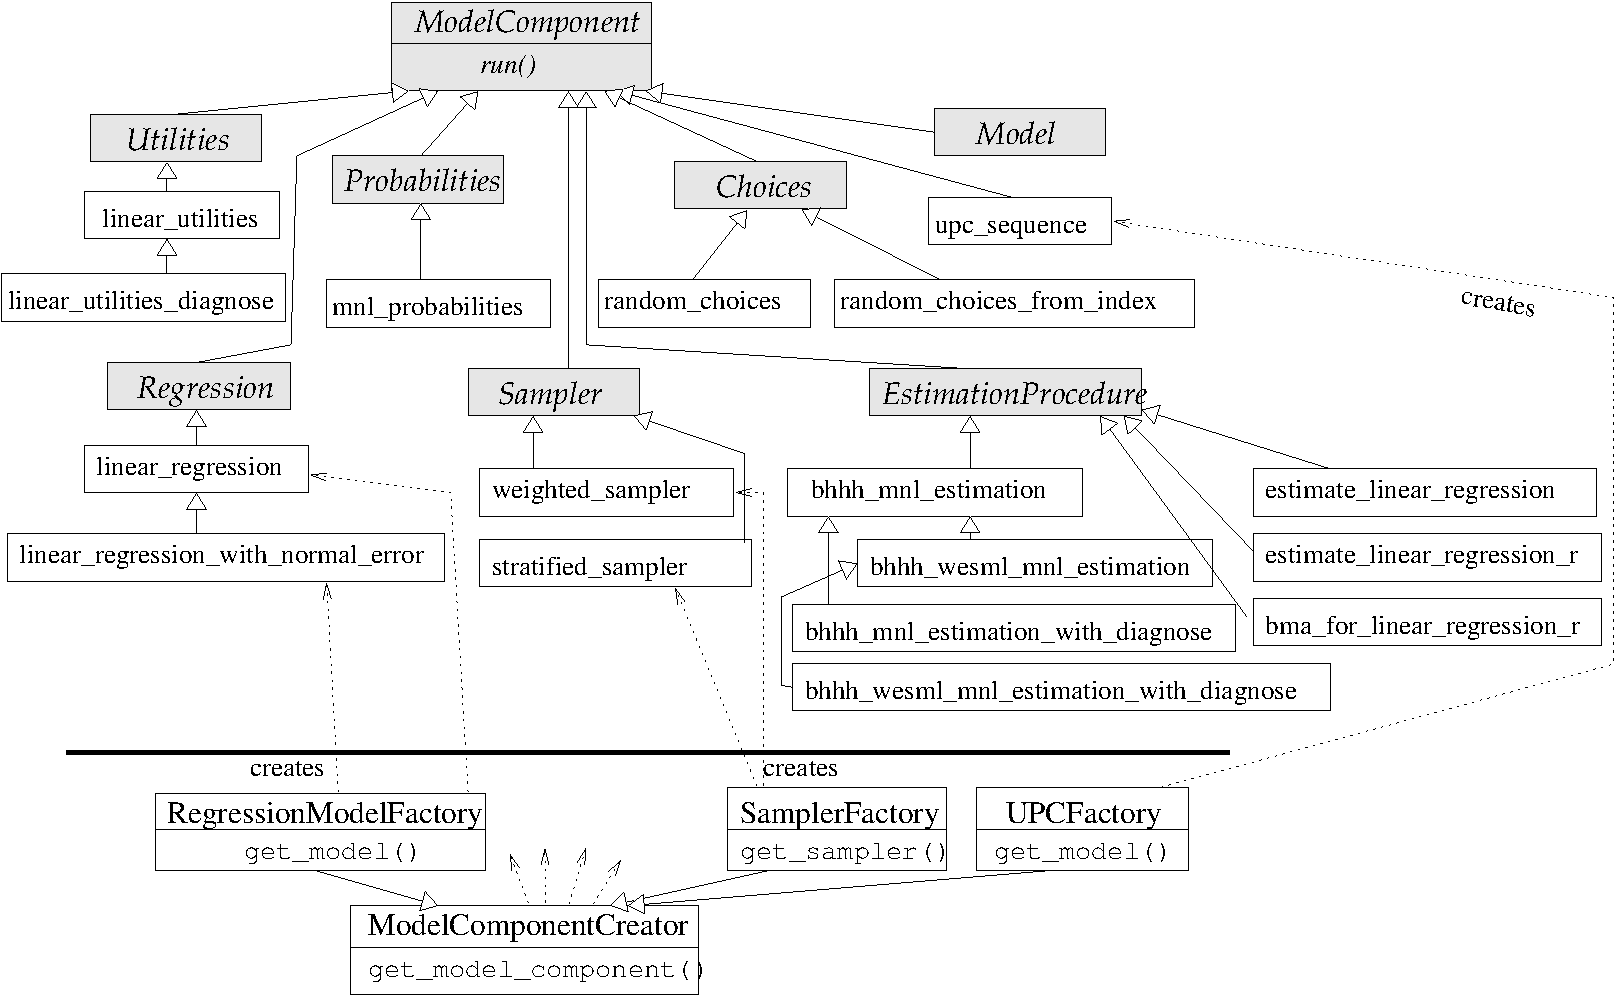
\includegraphics[scale=0.8, angle=-90]{images/corecomponents.pdf}
%end{latexonly}
\caption{\label{fig:model-components}\small Model components in Opus' \package{opus_core}.}
\htmlonly{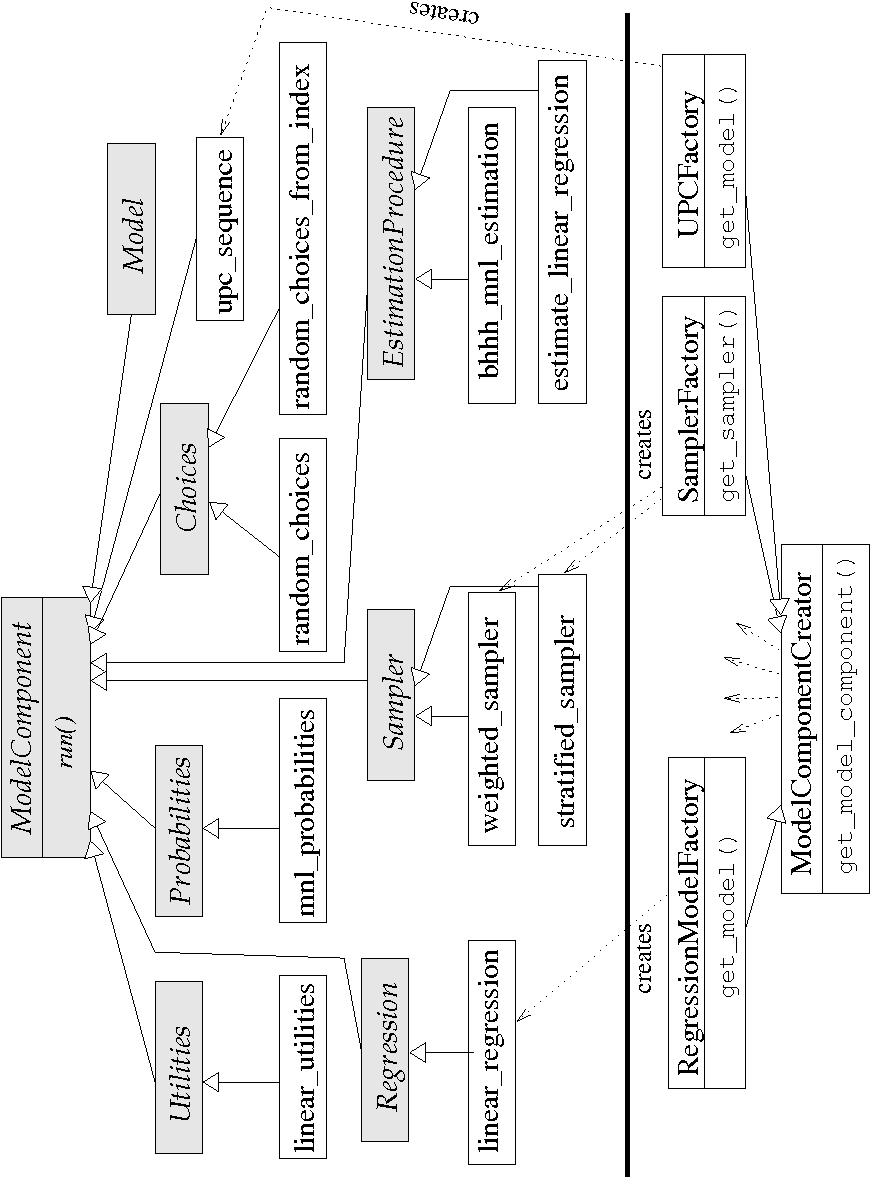
\includegraphics[scale=0.8, angle=-90]{images/corecomponents.jpg}}
\end{center}
\end{figure}

Instances of model components can be created using the class
\class{ModelComponentCreator}, by passing the class name into the method
\verb|get_model_component()|. In such a case the class name must be the same
as the module name. If it is not the case, one can use \class{ClassFactory}
for this purpose. There are a few child classes of
\class{ModelComponentCreator} implemented in \package{opus_core} for creating specific
model components.

\subsection{Utilities Class}
\label{sec:utilities}
\index{class!Utilities}

The \class{Utilities} class is used for computing utilities in
discrete choice modeling. In Opus \package{opus_core} there is one
\class{Utilities} class implemented -- {\bf linear_utilities} --
that computes linear utilities:
\[
U_{ni} = \sum_{j=1}^J \beta_{ij}x_{nij}\,.
\]
Here $i=1,\dots,I$ denotes the $I$ different alternatives, $n$ is an index for
observations (agents), $x$ denotes values of $J$ variables (including
constants) for each agent and alternative, and $\beta$ is a coefficient \coefficientsindex matrix
of size $I\times J$. The \verb|run()| method gets a 3-d array of data and a
2-d array of coefficients \coefficientsindex as arguments and returns a 2-d array of utilities.

\subsection{Probabilities Class}
\label{sec:probabilities}
\index{class!Probabilities}

The \class{Probabilities} class is an abstract class for computing
probabilities in the discrete choice modeling framework. Given
utilities $U$, the Opus \package{opus_core} class {\bf
mnl_probabilities} computes multinomial logit probabilities:
\[
P_{ni} = \frac{e^{U_{ni}}}{\sum_{j} e^{U_{nj}}}\,.
\]
Thus, the method \verb|run()| takes a 2-d array of utilities as an argument
(number of agents $\times$ number of alternatives) and returns a 2-d array of
probabilities (the same shape as utilities).

\subsection{Choices Class}
\label{sec:choices}
\index{class!Choices}

\class{Choices} is an abstract class for selecting choices according to given
probabilities in the discrete choice modeling framework. Opus package \package{opus_core} supports
two classes in this category. {\bf random_choices} returns an index of
randomly selected choices, one per observation. The number of alternatives is
simply derived from the second dimension of the array of probabilities, which
is passed as argument to the \verb|run()| method. {\bf
  random_choices_from_index} allows one to define an index array whose
elements are returned as the selected choices. This index array should be
contained in the argument \verb|resources| as an entry \verb|index|. This can be
useful for example if we are not dealing with the whole set of alternatives,
but rather with a subsampled set.

\subsection{upc_sequence Class}
\label{sec:upc-sequence}
\index{class!upc_sequence}

In the discrete choice modeling framework, there is a certain order of steps
that need to be evaluated, namely computing utilities, computing
probabilities and selecting choices. This class allows to perform these steps
using just one method call.

The class \class{upc_sequence} is composed by an object of \class{Utilities},
an object of \class{Probabilities} and an object of \class{Choices}. The
objects are passed to the constructor. Alternatively, one can use the
\class{UPCFactory} class, which creates an \class{upc_sequence} object from
names (character strings) of the components.

The \method{run()} method calls the \method{run()} methods of the component
classes in the order given above, passing results from one class to the next
one as input values. Thus, the method takes a 3-d array of data and a 2-d
array of coefficients \coefficientsindex as arguments and returns an array of choices.  Any of
the components can be eliminated by setting it to None. In such a case, the
components receive results of the previously running component as input and
the results of the very last running method is the return value of the
\method{run()} method of \class{upc_sequence}.

\subsection{Regression Class}
\label{sec:regression}
\index{class!Regression}

The \class{Regression} class is an abstract class for user defined classes
that can be used in the regression model. The class {\bf linear_regression}
implemented in \package{opus_core} computes outcome $Y$ as a linear combination of given
data $X$ and coefficients \coefficientsindex \boldmath $\beta$\unboldmath: $y_n = \sum_{j=1}^J
\beta_j x_{nj}$. Here, $J$ denotes the number of variables \variablesindex entering the
regression and $n$ is an index for observations. The \verb|run()| method takes
a 2-d array of data (of size number of observations $\times$ number of
variables) and a 1-d array of coefficients \coefficientsindex as arguments and returns a 1-d
array of outcome.

\subsection{EstimationProcedure Class}
\label{sec:estimation-procedure}
\index{class!EstimationProcedure}
%
This class is an abstract class for modules that implement estimation of
coefficients \coefficientsindex for one of the available models. {\bf bhhh_mnl_estimation}
implements the BHHH estimation algorithm for multinomial logit models and can
be plugged into the \class{ChoiceModel}. It gets a data array (of size number
of observations $\times$ number of alternatives $\times$ number of variables) \variablesindex
and an object \class{upc_sequence} as arguments. It uses the classes
\class{Probabilities} and \class{Utilities} contained in \class{upc_sequence}
for the maximum likelihood estimation. This assures that if
\class{bhhh_mnl_estimation} is plugged into the \method{estimate()} method of
\class{ChoiceModel} (Section~\ref{sec:choice-model}), the model will be
estimated by using the same code for computing utilities and probabilities as
the \verb|run()| method.  The third argument of the \verb|run()| method of
this class is of type \class{Resources} and must contain an entry
\verb|selected_choice| which is a 0-1 matrix of size number of observations
$\times$ number of alternatives. For each agent, it contains a 1 on a position
of the chosen alternative, otherwise 0s. Note that \class{ChoiceModel}
prepares and passes this matrix automatically.

{\bf estimate_linear_regression} performs a parameters estimation via the
least squares method. It gets a data array (of size number of observations
$\times$ number of variables), \variablesindex an instance of class \class{Regression} (not
used in this module) and an object \class{Resources} as arguments. The last
argument must contain an entry \verb|outcome| which is a 1-d array of an outcome
for each observation. This class can be plugged into the
\class{RegressionModel} which takes care of all arguments.

The estimation modules return a dictionary, with entries \verb|estimators| and
\verb|standard_errors|. These contain arrays of estimated coefficients \coefficientsindex and their
standard errors, respectively. An entry \verb|other_measures| is a dictionary
which should contain additional measures of the estimates, i.e. their values
should be arrays of the same size as estimators. The two estimation modules
in \package{opus_core} return here one entry, namely the \verb|t_statistic|. The last entry in
the dictionary returned by the modules, \verb|other_info|, is a dictionary
containing additional information about the estimation. Its values don't
follow any restriction on type and size. Thus, these can be also single values,
such as likelihood ratio test statistics, degrees of freedom, $R^2$ etc.

%% \subsection{sampling_toolbox}
%% \label{sec:samplingtoolbox} The sampling_toolbox is a collection of
%% sampling functions built upon numpy.  It provides equal
%% probability sampling with and without replacement
%% ({\it{sample_replace}} and {\it{sample_noreplace}} respectively),
%% unequal probability sampling with and without replacement ({\it{probsample_replace}}
%% and {\it{probsample_noreplace}} respectively), stratified sampling ({\it{stratifiedsample}}),
%% 2d sampling ({\it{prob2dsample}}), sampling (Monte Carlo(MC) or max_prob) ``choice'' from
%% a 2d probability array({\it{sample_choice}}), as well as functionality of normalization of
%% weight or probability ({\it{normalize}}) and finding duplicates ({\it{find_duplicates}} and
%% {\it{find_duplicates_others}}) in array.

%% Please refer to its source code sampling_toolbox.py in opus_core for detail usage.

\subsection{Sampler Class}
\label{sec:sampler}
\index{Sampler}
\index{class!Sampler}

The \class{Sampler} class is an abstract class for sampling alternatives for agents.
It returns 2-d array with rows representing agents and columns representing sampled
alternatives. It is not directly used in any Opus model, but it is a building
block that can be used in models of other packages. For example, we made a
heavy use of this component in the \package{urbansim} package for creating sampled
alternative set for agents in \class{ChoiceModel}.

\subsubsection{weighted_sampling}
\index{class!weighted_sampling}

{\bf weighted_sampling} is a child class of \class{Sampler} class.
It randomly samples alternatives from choice population with
probability proportion to their weights. Its run method accepts the
following arguments:
\begin{description}
\item[dataset1] - an instance of \class{Dataset}, \datasetindex to be used as agent set.
\item[dataset2] - an instance of \class{Dataset}, \datasetindex to be used as choice set.
\item[index1] - indices of \verb|dataset1| for whom alternatives are sampled.
If it is not given, all elements of dataset1 are used.
\item[index2] - indices of \verb|dataset2| from which alternatives are
sampled. If it is not given, all elements of dataset2 are used.
\item[sample_size] - number of alternatives sampled.
\item[weight] - an array used as weight for elements of dataset2 in unequal
probability sampling; it has to be either of None, or of the same size as index2 or
dataset2. If it is not given, sampling is proceeded with equal probability.
\item[include_chosen_choice] - whether agents' chosen choice will be included in
the return results. If it's true, the chosen choices are in the first column of
the return results.
\item[resources] - an instance of \class{Resources} that can be used to pass any of
the above arguments to run method.
\end{description}

\subsubsection{stratified_sampling}
\index{class!stratified_sampling}

{\bf stratified_sampling} is a child class of \class{Sampler} class.
It randomly samples alternatives from choice population according to
their stratum setting. Its run method accepts the following
arguments:
\begin{description}
\item[dataset1] - an instance of \class{Dataset}, \datasetindex to be used as agent set.
\item[dataset2] - an instance of \class{Dataset}, \datasetindex to be used as choice set.
\item[index1] - indices of \verb|dataset1| for whom alternatives are sampled.
If it is not given, all elements of dataset1 are used.
\item[index2] - indices of \verb|dataset2| from which alternatives are
sampled. If it is not given, all elements of dataset2 are used.
\item[stratum] - an array indicates the stratum id for elements of dataset2; it has
to be either of None, or of the same size as index2 or dataset2. If it's not given,
all elements are treated as in 1 stratum.
\item[weight] - like in weighted_sampling, weight is an array used as weight
for elements of dataset2 in unequal probability sampling; it has to be either
of None, or of the same size as index2 or dataset2. If it is not given, sampling
is proceeded with equal probability.
\item[sample_size] - number of alternatives sampled from one stratum; default value is 1.
\item[sample_size_from_chosen_stratum] - number of alternatives sampled from agent's chosen stratum.
If it's None, it's equal to value specified by sample_size or sample|_rate.
\item[sample_rate] - calculate number of alternatives sampled from one stratum by multiplying this rate with
number of observations in this stratum. If both sample_rate and sample_size are specified, use sample_rate.
\item[include_chosen_choice] - whether agents' chosen choice will be included in
the return results. If it's true, the chosen choices are in the first column of
the return results.
\item[resources] - an instance of \class{Resources} that can be used to pass any of
the above arguments to run method.
\end{description}


\section{Specification and Coefficients}
\label{sec:specification-coefficients}
%
\subsection{Specification}
\index{Specification}
\index{class!EquationSpecification}
%
\label{sec:specification}
Often, models are specified by a set of variables. \variablesindex These are connected to a
set of coefficients \coefficientsindex calibrated to the observed data. Opus defines a class for
such specification, called \class{EquationSpecification}.

\subsubsection{Initialization}
The constructor of \class{EquationSpecification}
takes the following arguments:
\begin{description}
\item[variables] - an array of variable \variablesindex names.
\item[coefficients] - an array  of coefficient \coefficientsindex names.
\item[equations] - an array of equations.
\item[submodels] - an array of submodels.
\item[in_storage] - an object of class \class{Storage} for loading
  specification from a storage.
\item[out_storage] - an object of class \class{Storage} for specification output.
\end{description}
The arrays \verb|variables| \variablesindex and \verb|coefficients| \coefficientsindex must have the same size.
If \verb|submodels| and \verb|equations| are not omitted, they too must have
the same lengt as \verb|variables|. \variablesindex It is interpreted as the $i$-th variable \variablesindex
is connected to the $i$-th coefficient \coefficientsindex in the $i$-th equation (if there are
any) in the $i$-th submodel (if there are any). Values of \verb|equations| and
\verb|submodels| should be strictly positive integers. Coefficients \coefficientsindex should
have different names across equations, i.e. if there would be $i$ and $j$ for
which the \verb|coefficients[i]==coefficients[j]| \coefficientsindex and
\verb|equations[i]<>equations[j]| and \verb|submodels[i]==submodels[j]|, it
would lead to errors when connecting specification and coefficients. \coefficientsindex

All arguments are set as class properties. \verb|in_storage| and
\verb|out_storage| are not used in the constructor.

\subsubsection{Loading from and Writing into Storage}
%
One can also omit the arguments in the constructor and load the specification
from a storage, using the method \method{load()}. It takes the following
arguments:
\begin{description}
\item[resources] - an object of class \class{Resources}. If the remaining
  arguments are given, they will have priority over entries of the same name
  in \verb|resources|.
\item[in_storage] -  an object of class \class{Storage} that overwrites the
  one given in the constructor.
\item[in_table_name] - name of the table/file where the specification should
  be loaded from.
\item[variables] - if this argument is given, it serves as a filter for the
  variables \variablesindex loaded from the store.
\end{description}
For each of the class properties variables, \variablesindex coefficients, \coefficientsindex equations, and
submodels, respectively, a table column is expected on the storage. The column
names are given in the \verb|resources| entries \verb|field_variable_name|,
\verb|field_coefficient_name|, \verb|field_equation_id|, and \verb|field_submodel_id|,
respectively. Default values are \verb|'variable_name|, \variablesindex \verb|'coefficient_name|, \coefficientsindex
\verb|'equation_id|, and \verb|'sub_model_id|.

The variables \variablesindex and coefficients \coefficientsindex are stored in the class attributes \attributesindex
\verb|variables| \variablesindex and \verb|coefficients|. \coefficientsindex Equations and submodels are stored
only if their maximum value is not negative.

To store a specification into a storage, use the method
\method{write(resources, out_storage, out_table_name)}. The behavior is
analogous to the \method{load()} method. If equations or/and submodels are not
used, the method stores values $-2$ in those columns.


\subsection{Coefficients}
\coefficientsindex
\label{sec:coefficients}
\index{class!Coefficients}
%
Coefficients \coefficientsindex can be managed by the class \class{Coefficients}. \coefficientsindex Its behavior
is similar to the one of \class{EquationSpecification}.

\subsubsection{Initialization}
The constructor takes the following arguments:
\begin{description}
\item[names] - an array of coefficient \coefficientsindex names.
\item[values] - an array of coefficient \coefficientsindex values (of the same size as
  \verb|names| if not empty).
\item[standard_errors] - an array of standard errors of coefficients \coefficientsindex (of the
  same size as \verb|names| if not empty).
\item[submodels] - an array of submodels (of the same size as \verb|names| if
  not empty).
\item[in_storage] - an object of class \class{Storage} for loading
  coefficients \coefficientsindex from a storage.
\item[out_storage] - an object of class \class{Storage} for coefficients \coefficientsindex
  output.
\item[other_measures] - a dictionary for other coefficient \coefficientsindex measures, such as
  t-values. Keys are the names of the measures, values are arrays or of
  the same size as \verb|names|.
\item[other_info] - dictionary storing other information about the
  coefficients, \coefficientsindex such as goodness of fit values.
\end{description}
The arguments are interpreted as the coefficient \coefficientsindex of $i$-th name has the $i$-th
value, optionally the $i$-th standard error and is used in $i$-th
submodel. This also applies to \verb|other_measures|. Note that since
equations are not used here, there has to be coefficients \coefficientsindex with different names
for different equations, defined in the specification.

All arguments are set as class properties. \verb|in_storage| and
\verb|out_storage| are not used in the constructor.

%
\subsubsection{Loading from and Writing into Storage}
%
The method \method{load()} is similar to the one defined in
\class{EquationSpecification}. It take as arguments:
\begin{description}
\item[resources] - an object of class \class{Resources}. If the remaining
  arguments are given, they will have priority over entries of the same name
  in \verb|resources|.
\item[in_storage] -  an object of class \class{Storage} that overwrites the
  one given in the constructor.
\item[in_table_name] - name of the table/file where the coefficients \coefficientsindex should
  be loaded from.
\end{description}
For each of the class properties names, values, standard errors, and
submodels, respectively, a table column is expected on the storage. There can
be other fields stored too. The column names are given in the \verb|resources|
entries \verb|field_coefficient_name|, \coefficientsindex \verb|field_estimate|,
\verb|field_standard_error|, and \verb|field_submodel_id|, respectively. Default
values are \verb|variable_name|, \variablesindex \verb|coefficient_name|, \coefficientsindex \verb|equation_id|, and
\verb|sub_model_id|. If there are other fields in the table, the column names are
given in the entry \verb|other_fields| which is a list of character strings. The
default value is \verb|['t_statistic', 'p_value']|.

To store coefficients \coefficientsindex into a storage, use the method
\method{write(resources, out_storage, out_table_name)}. The behavior is
analogous to the \method{load()} method.

The class also allows to create a coefficient \coefficientsindex table in the \LaTeX
format. Method \method{make_tex_table()} accepts as arguments the file name
(without `.tex'), optionally the directory path and headers for each column.

\subsection{Specified Coefficients}
\label{sec:specified-coefficients}
\index{class!SpecifiedCoefficients}
%
In order to connect a specification with coefficients, \coefficientsindex Opus uses the class
\class{SpecifiedCoefficients}. Its method \method{create()} takes an instance
of class \class{Coefficients} and an instance of class
\class{EquationSpecification} and creates arrays of coefficient \coefficientsindex values,
standard errors and other measures. The shape of those arrays is such that
they can be easily combined with data arrays when connecting coefficients \coefficientsindex to
variable \variablesindex values. In particular they have three dimensions, number of
equations, number of variables \variablesindex and number of submodels.

For working with single submodels, there is a child class of
\class{SpecifiedCoefficients}, \coefficientsindex called
\class{SpecifiedCoefficientsFor1Submodel}, \coefficientsindex that is initialized by passing the
parent object and the submodel number.

Those classes are created and used by the two \package{opus_core} models, regression model
for computing the regression and the choice model for computing the utilities.

\section{Other Classes}
%
\subsection{Dataset Pool}
\label{sec:core-dataset-pool}
\index{dataset pool}
%
A class called \class{DatasetPool} is design to maintain a 'pool' of datasets. It is mainly used when
computing variables. Therefore in most cases, it will be only needed if the \class{Dataset} method
\method{compute_variables()} is used (for which an instance of \class{DatasetPool} is passed as an argument) in order
to have external datasets available that are required by the various variable implementations
 (see an example in Section~\ref{sec:variableconcept}).

The class is initialized by passing arguments:
\begin{description}
\item[package_order] - a list of packages that are used for finding the corresponding dataset class. Default is an empty list.
\item[package_order_exception] - a dictionary of exceptions from the \verb|package_order| as pairs dataset name
and list of packages for that dataset. Default is an empty dictionary.
\item[storage] - an object of class \class{Storage} that contains data of datasets to be included in pool. Default is \verb|None|.
\end{description}
One can add a dataset into the pool using the method \\
\method{_add_dataset(dataset_name, dataset)}, \\
or by
passing multiple datasets in one dictionary using the method \\
\method{add_datasets_if_not_included(datasets_dict)}.

A dataset can be accessed by the method \\
\method{get_dataset(dataset_name, dataset_arguments)}\\
 where the second argument is optional.
If a dataset of the given name is included in the pool, it is returned. Otherwise, the class creates a Dataset object with
data from the storage that was passed in the initialization. In order to create the appropriate Dataset class, it is searched
for a module called {\em dataset_name}\verb|_dataset.py| which should contain a class called {\em DatasetName}\verb|Dataset|.
The \class{DatasetPool} class searches for this module in the directory \file{datasets} of packages given in the initialization argument
'package_order'.

\subsection{ModelGroup and ModelGroupMember}
%
\label{sec:model-group}
\index{model group}
%
These two classes are designed to be used in models that are considered as model groups, i.e. models that are to be run
multiple times, each time on different subsets of one dataset.

A model group is defined by the following:
\begin{itemize}
\item There must be a dataset whose one attribute defines the names of the group members.
These names must be unique within the dataset.
We will call this dataset and its attribute {\em grouping dataset} and {\em grouping attribute} respectively.
Values of the unique identifier of the grouping dataset will be called  {\em member codes}.
\item A dataset that is going to be subset for running the model member on must contain an attribute whose values
represent the member codes. We will call this attribute {\em agents grouping attribute}.
\end{itemize}

Example: Suppose we would like to run a model on a 'job' dataset, subset according to its building type. Then
our grouping dataset, say 'job_building_type', can contain the following data:
\begin{verbatim}
id	name
1	'commercial'
2	'industrial'
3	'residential'
\end{verbatim}
The attribute 'name' is our grouping attribute, values of the 'id' attribute are member codes.
The dataset 'job' contains an attribute, say 'building_type' that has
value 1 for all commercial jobs, 2 for all industrial and 3 for all residential jobs. 'building_type' is then the
agents grouping attribute.

The class \class{ModelGroup} is initialized by
\begin{description}
\item[dataset] - Object of class \class{Dataset} that is the grouping dataset.
\item[grouping_attribute] - Name of the grouping attribute.
\end{description}
The class offers useful methods for accessing member names and codes of this group.

The class \class{ModelGroupMember} is initialized by
\begin{description}
\item[model_group] - An object of class \class{ModelGroup}.
\item[member_name] - Name of this specific member. It must be contained in the grouping attribute of 'model_group'.
\end{description}
A model that uses this class should use the method \method{set_agents_grouping_attribute(attribute)} to set
the agents grouping attribute. Then the class can be used for subsetting any dataset according to the member codes,
e.g. by the method \method{get_index_of_my_agents(dataset, index)} which selects those entries from the given index that
correspond to this group member.

\subsection{GeneralResources, SessionConfiguration, Configuration and Resources}
\label{sec:resources} \index{Configuration} \index{Resources} \index{GeneralResources}
%
Opus implements a few classes that are used for configuration of objects.
\begin{description}
\item[GeneralResources] - it is a python \pythonindex dictionary with some additional methods.
\item[SessionConfiguration] - a singleton (child of \class{GeneralResources} that is to be configured
        with global settings for a user's session.  Requires parameter
        \verb|in_storage| to not be \verb|None| if creating a new instance, so
        SessionConfiguration knows from where to get the data for any dataset it
        creates.
\item[Configuration] - it is a child of \class{GeneralResources} that implements a hierarchical
        representation of the user-specified parameters and settings.
\item[Resources] - it is a child of \class{Configuration}. It has access to the
\class{SessionConfiguration}.
\end{description}

%%% Local Variables:
%%% mode: latex
%%% TeX-master: "userguide"
%%% End:

% LocalWords:  tex borning uninstall Dataset SimulationState AttributeCache Un
% LocalWords:  MySQL versioning gridcell un VariableName AttributeBox rpy ij ln
% LocalWords:  matplotlib openev OpenEV DatasetSubset indices InteractionDataset attr
% LocalWords:  ChoiceModel attrtype valuetypes mysql Bool
% LocalWords:  StorageFactory columnwise txt urbansim DDD powDDD gridcells faz
% LocalWords:  numpy py VariableFactory UInt pre ds ChunkModel chunked upc
% LocalWords:  RegressionModel ChunkSpecification submodel submodels config ni
% LocalWords:  EquationSpecification RegressionModelFactory ClassFactory nij nj
% LocalWords:  ModelComponentCreator mnl logit subsampled UPCFactory bhhh bla
% LocalWords:  EstimationProcedure UrbanSim SpecifiedCoefficients userguide
% LocalWords:  SpecifiedCoefficientsFor
